\section[Unaligned 2-D Images and Angular Synchronization]{Factoring Out Symmetries in Two--Dimensional~Images Using~Angular~Synchronization}

\begin{frame}{Images Instead of Concentration Profiles}
	
	\centering
    As a preprocessing step, we have to take fluorescent images of the embryo~cross-sections and convert them to concentration profiles on a ring\\
    \centering
    \begin{tikzpicture}
        \node (dpERKimage) {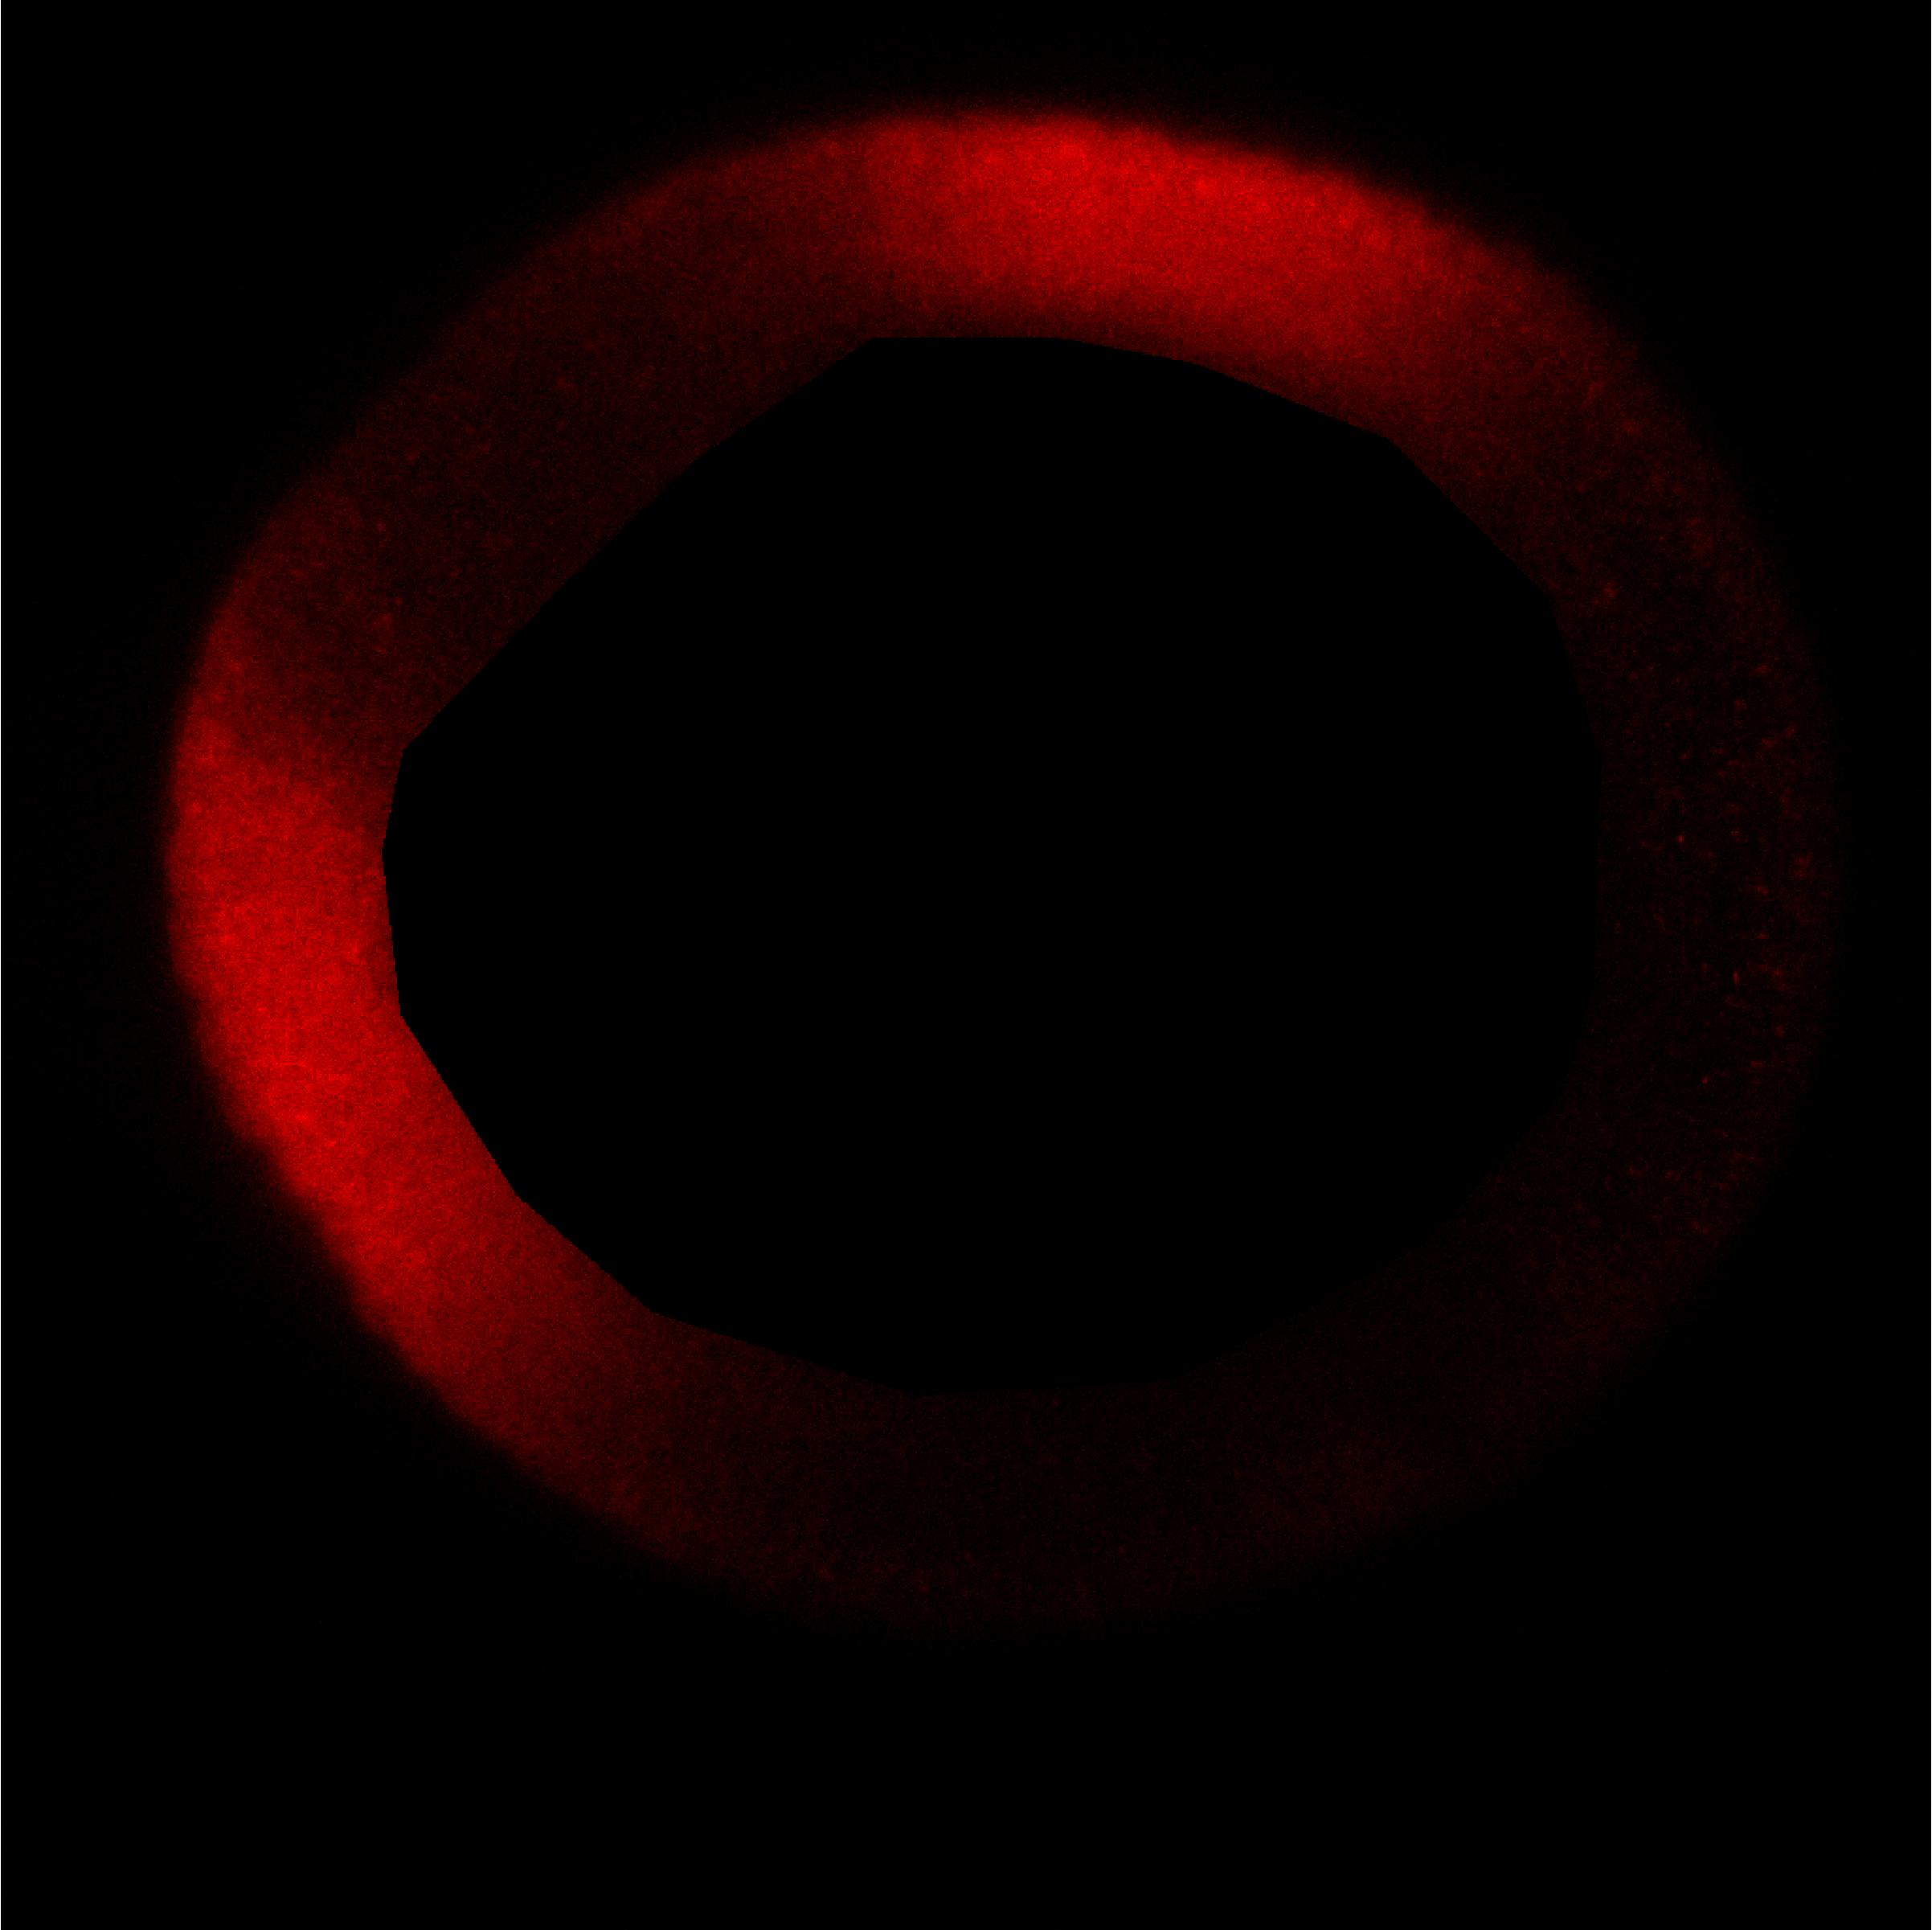
\includegraphics[width=0.3\textwidth]{drosophila_dpERK}};
        		\draw[gray,<->] (dpERKimage.south west) --  (dpERKimage.south east) node[below,midway] { \tiny $100 \mu m$};

        \node[right=of dpERKimage] (dpERKprofile) {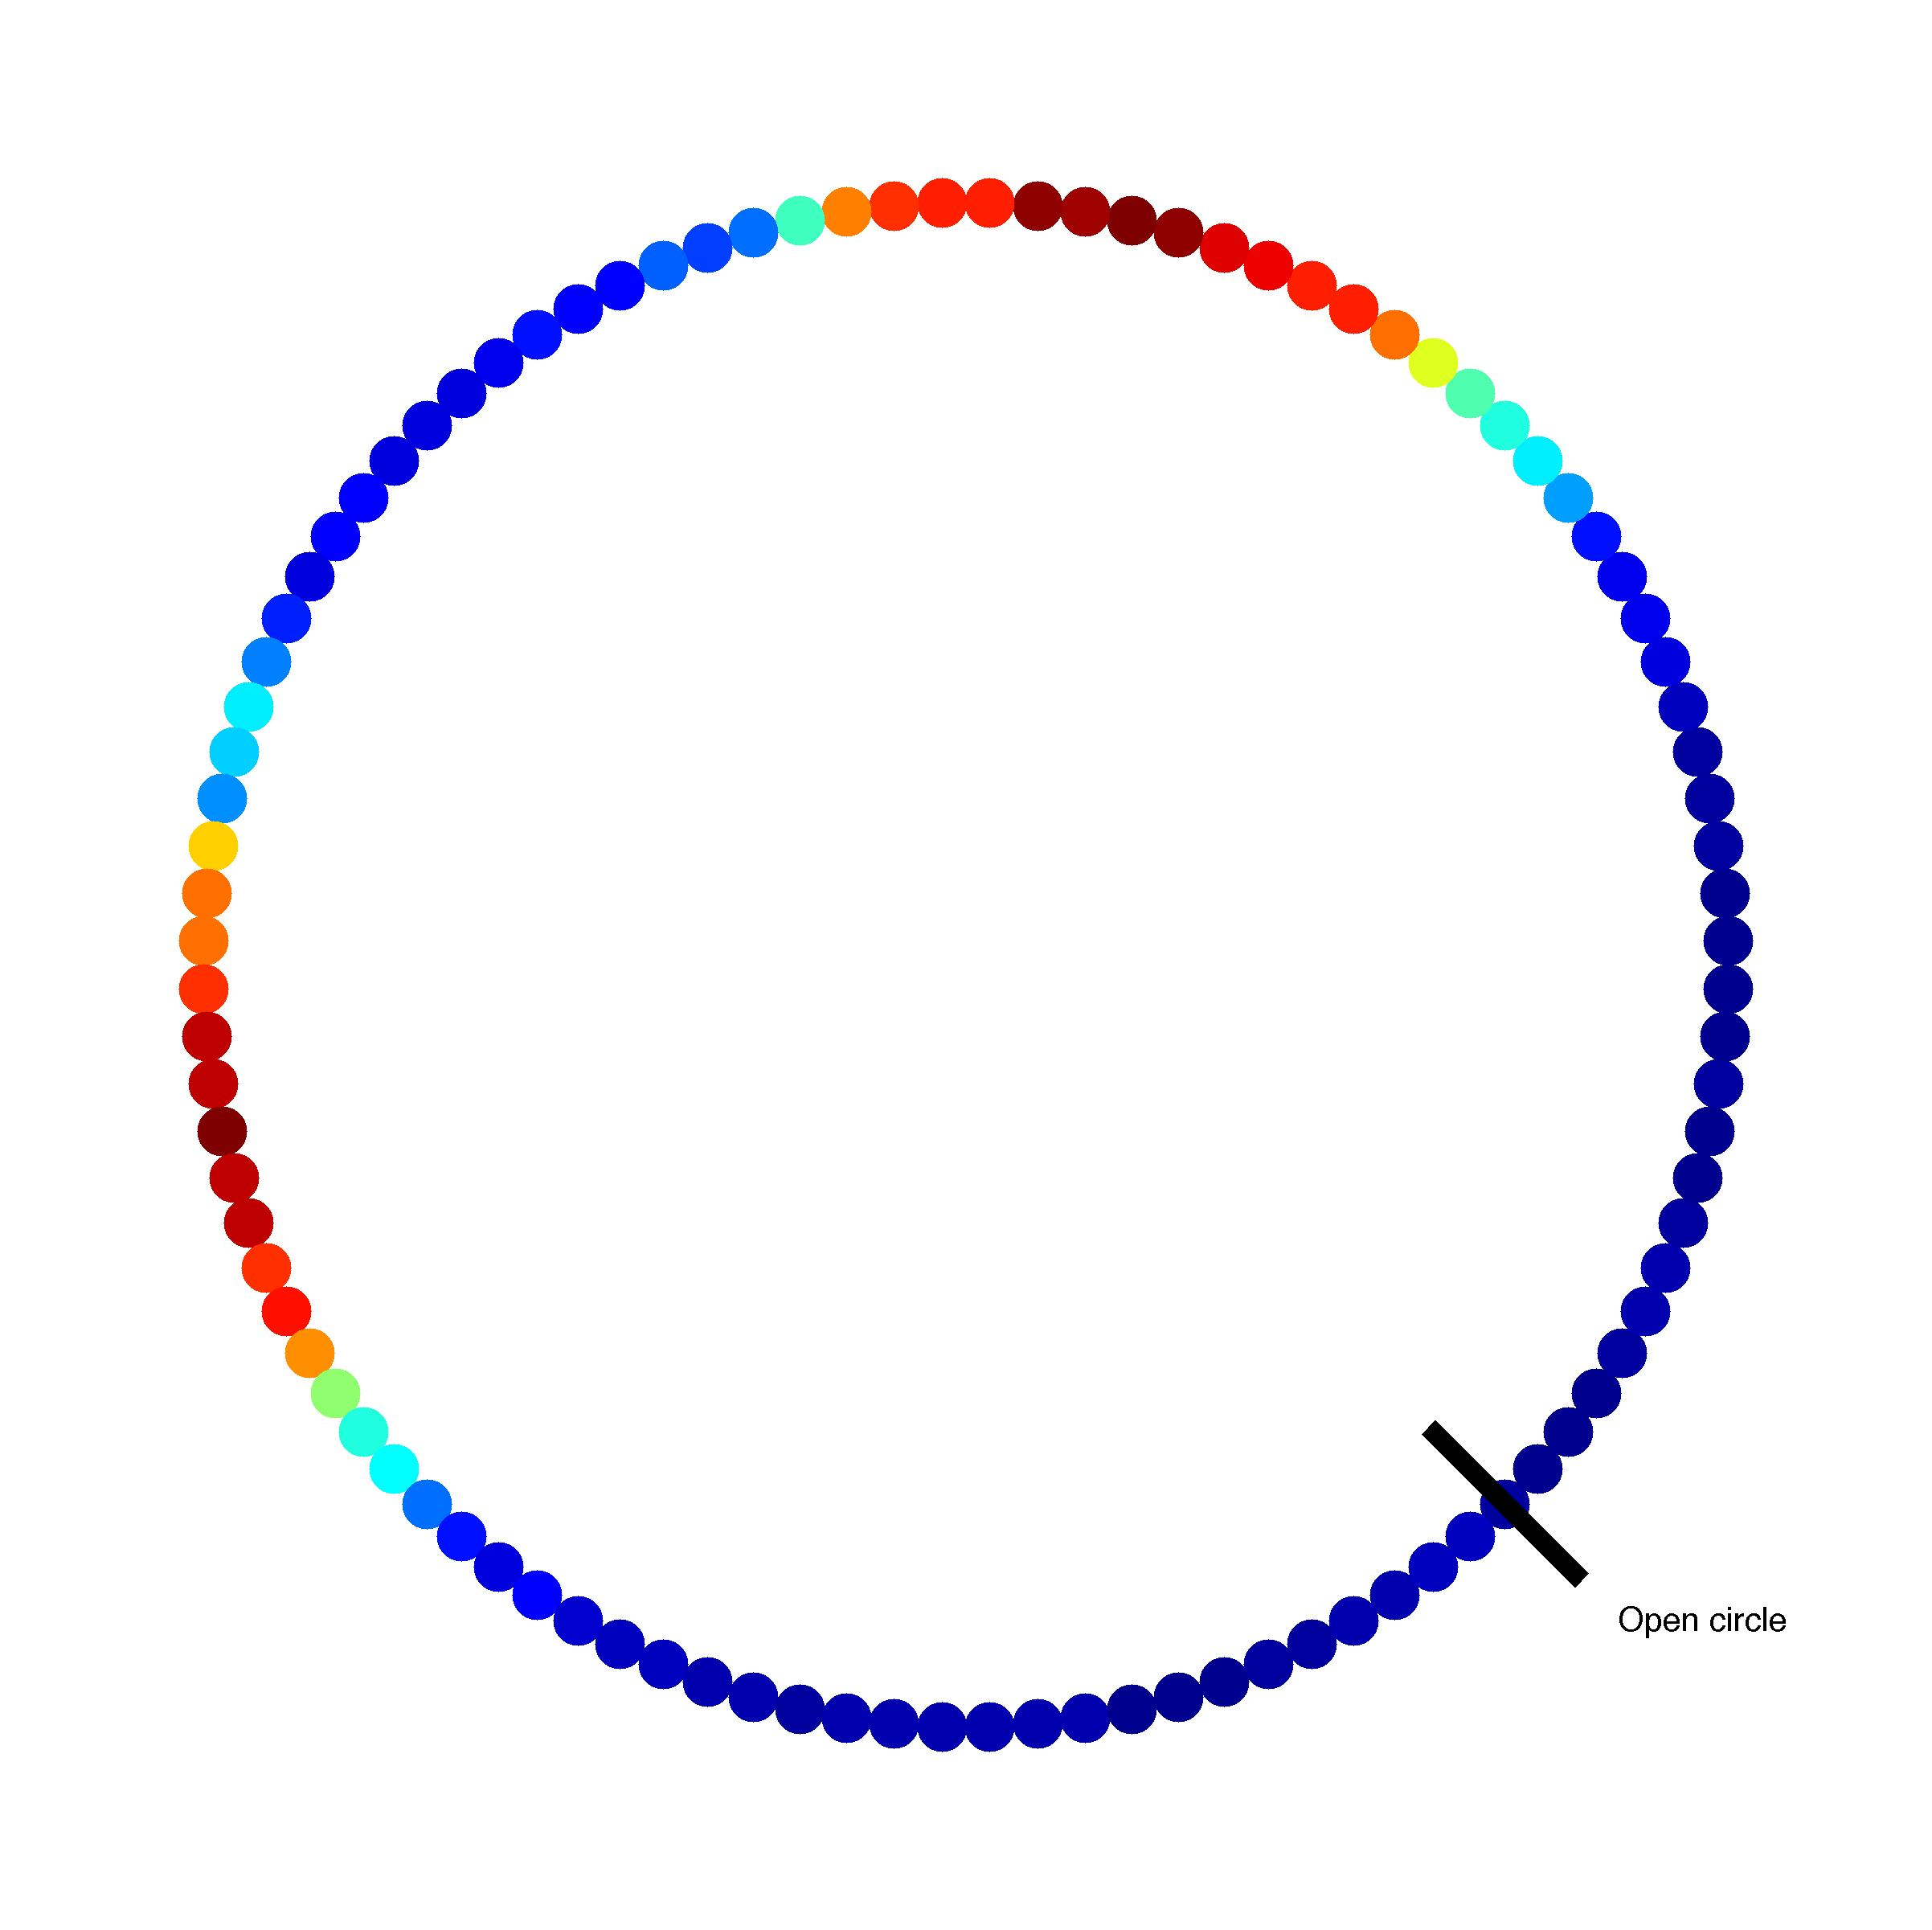
\includegraphics[width=0.3\textwidth]{circle_profile}};
        \draw[->] (dpERKimage)--(dpERKprofile);
    \end{tikzpicture}
    
    However, we could do the same analysis with {\bf raw images} instead of the concentration profiles to extract the dynamics
    
    We must now synchronize/align the images under all {\bf translations and rotations}
    
\end{frame}

\begin{frame}{Alignment of Two-Dimensional Images}
    We first align and order the images using vector diffusion maps\\
    
    \centering
    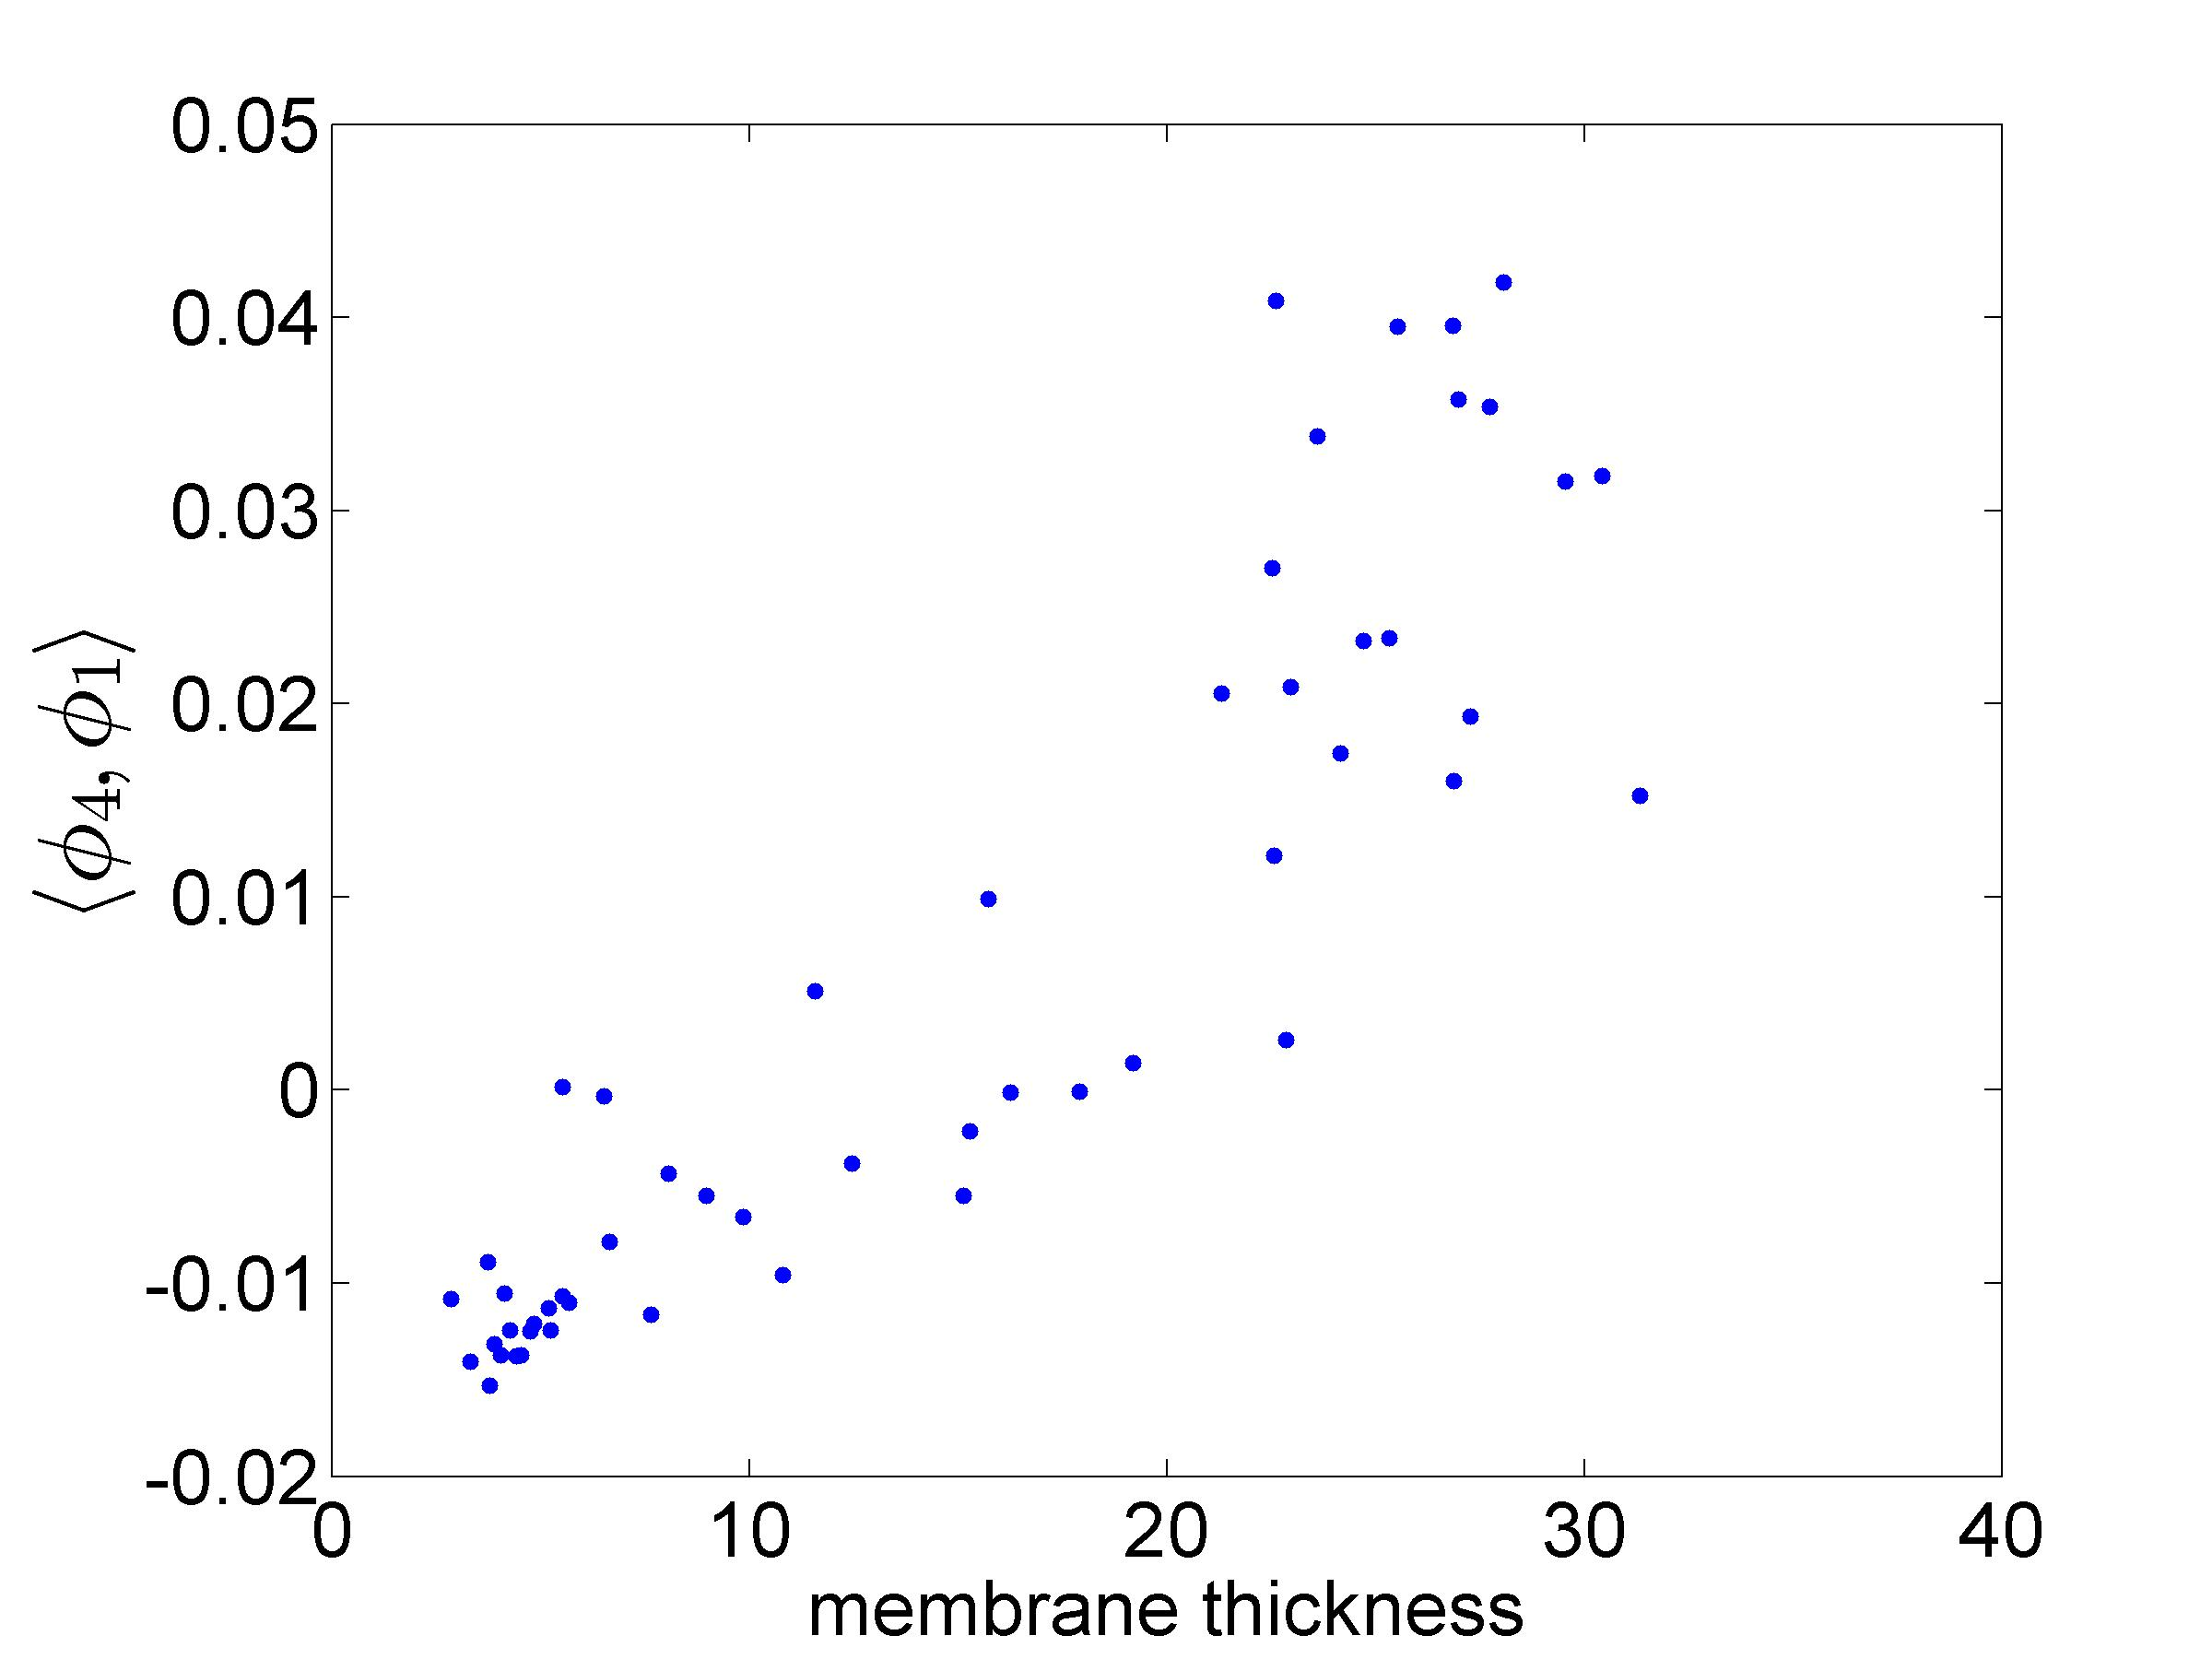
\includegraphics[width=0.5\textwidth]{vdm_2d_time_corr}\\
    
\includegraphics[width=0.15\textwidth]{dpERK_vdm_1}
    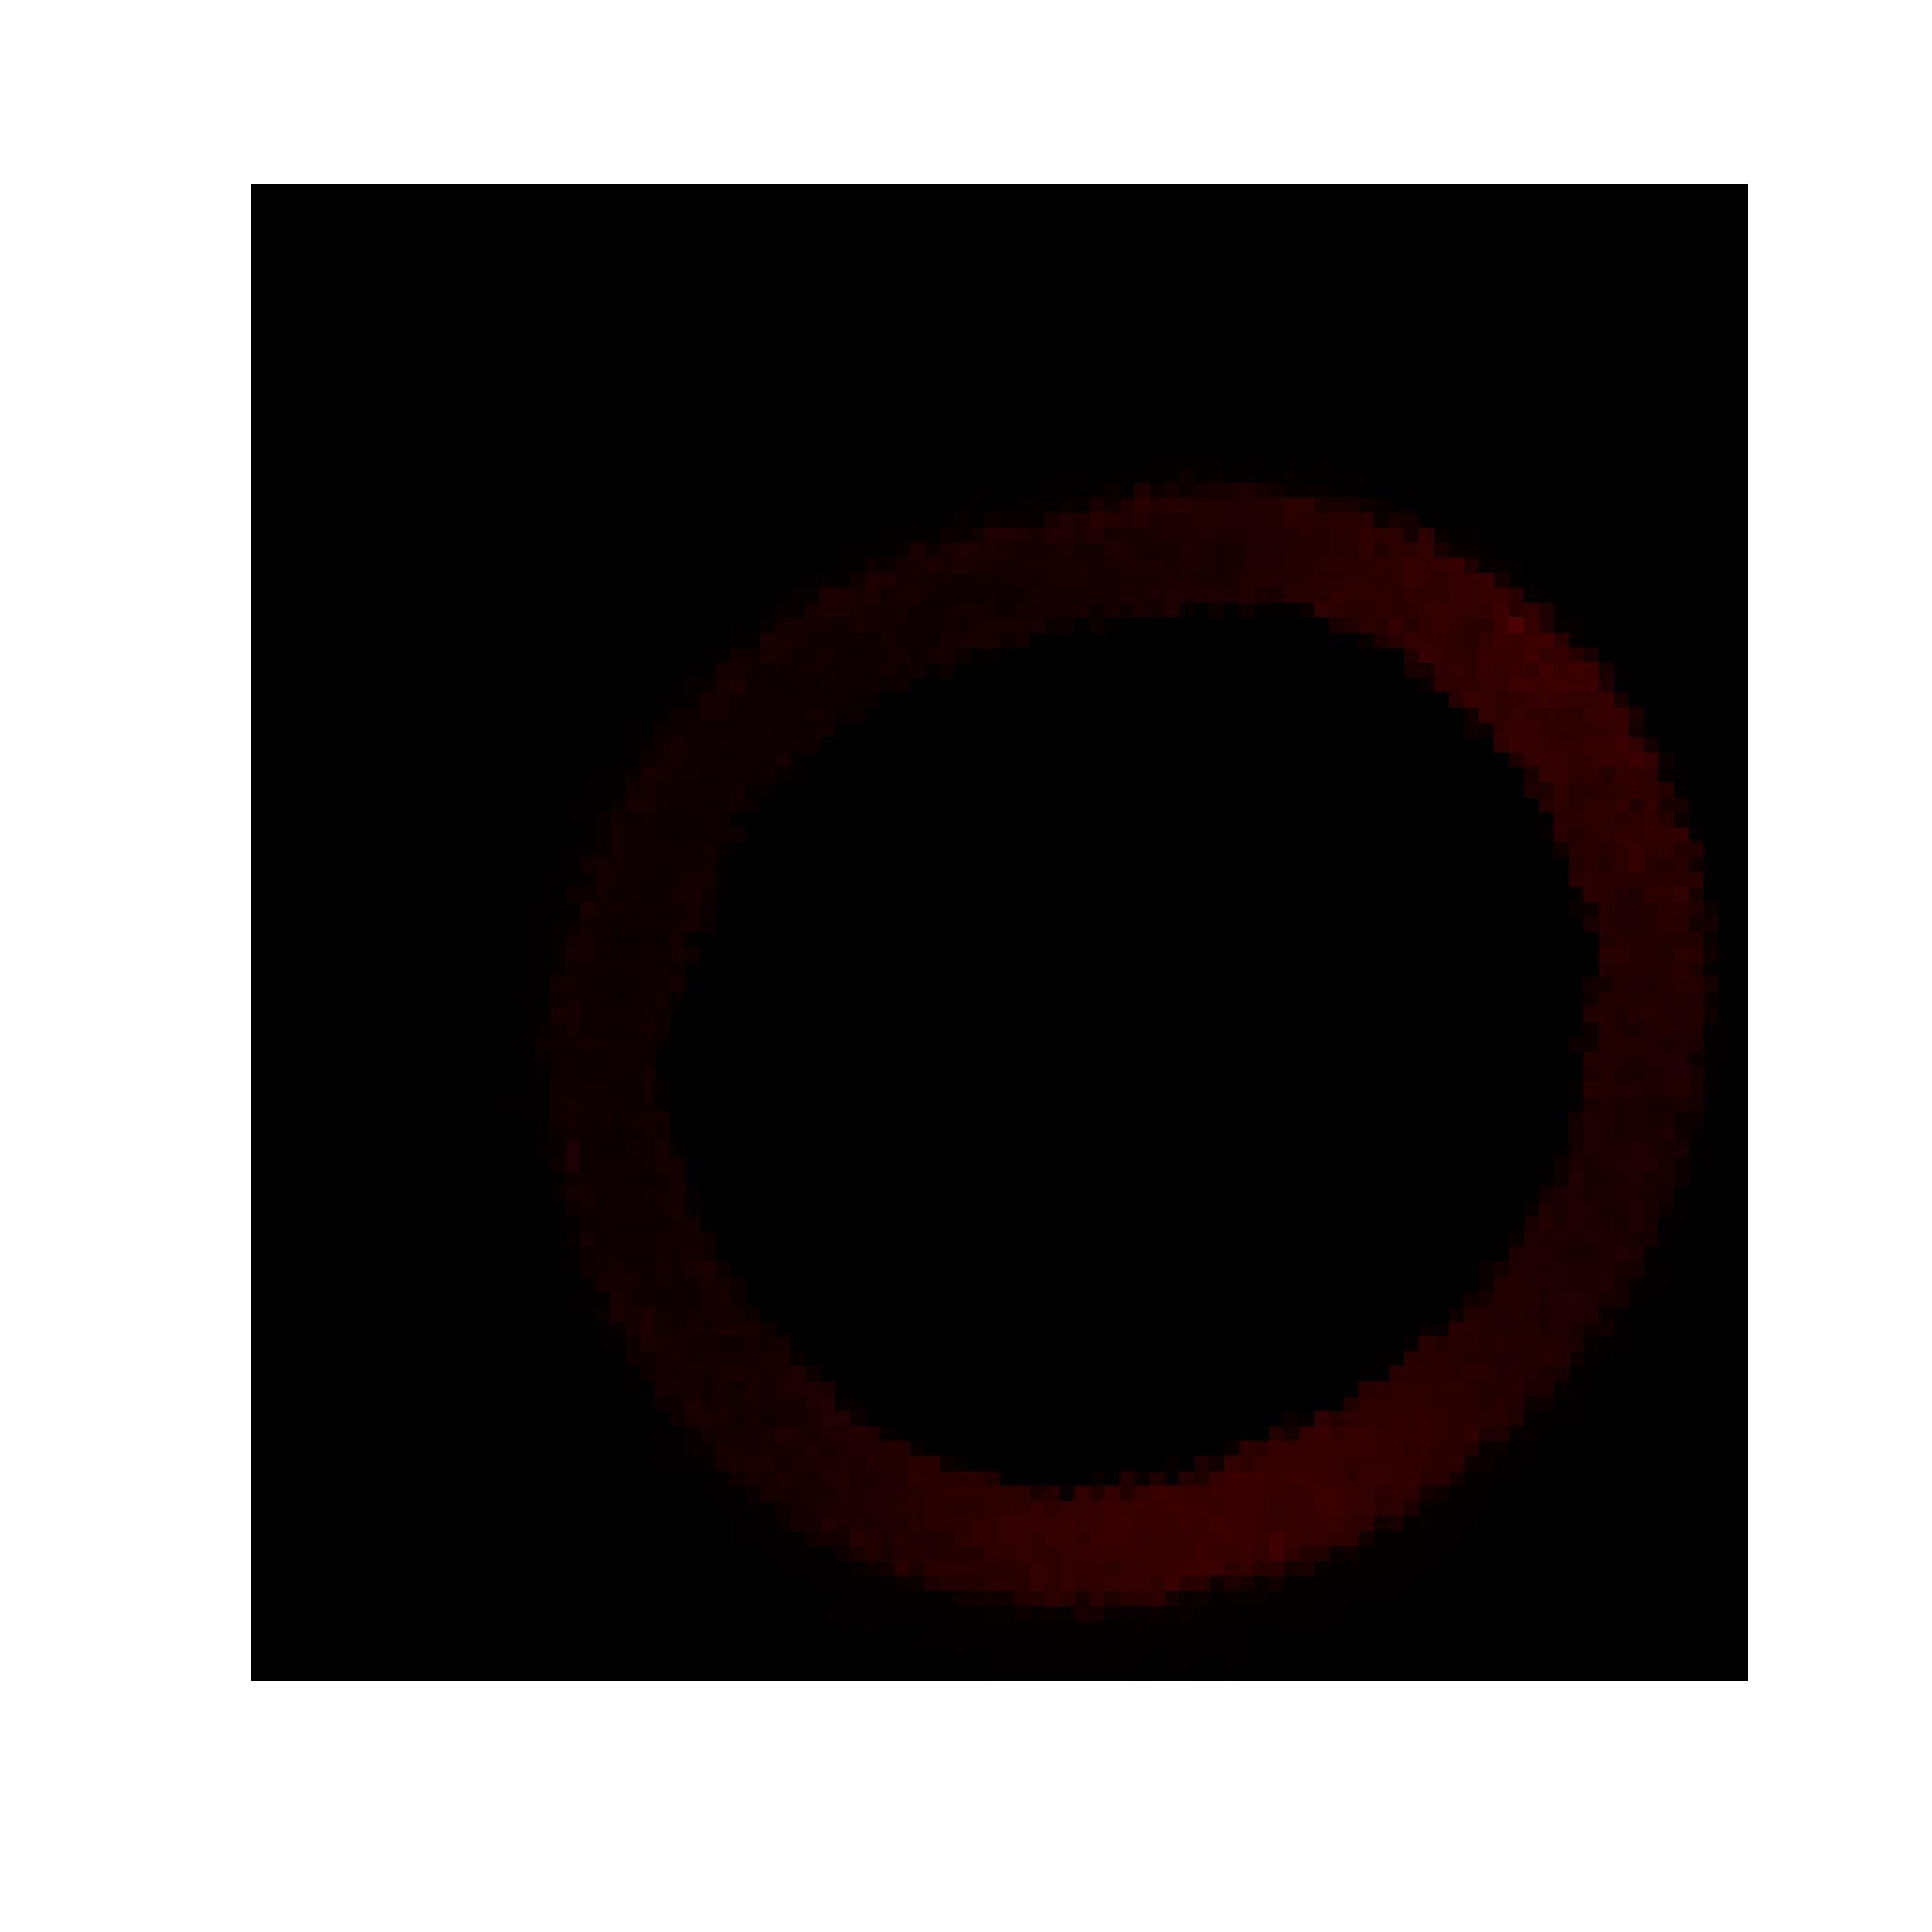
\includegraphics[width=0.15\textwidth]{dpERK_vdm_2}
    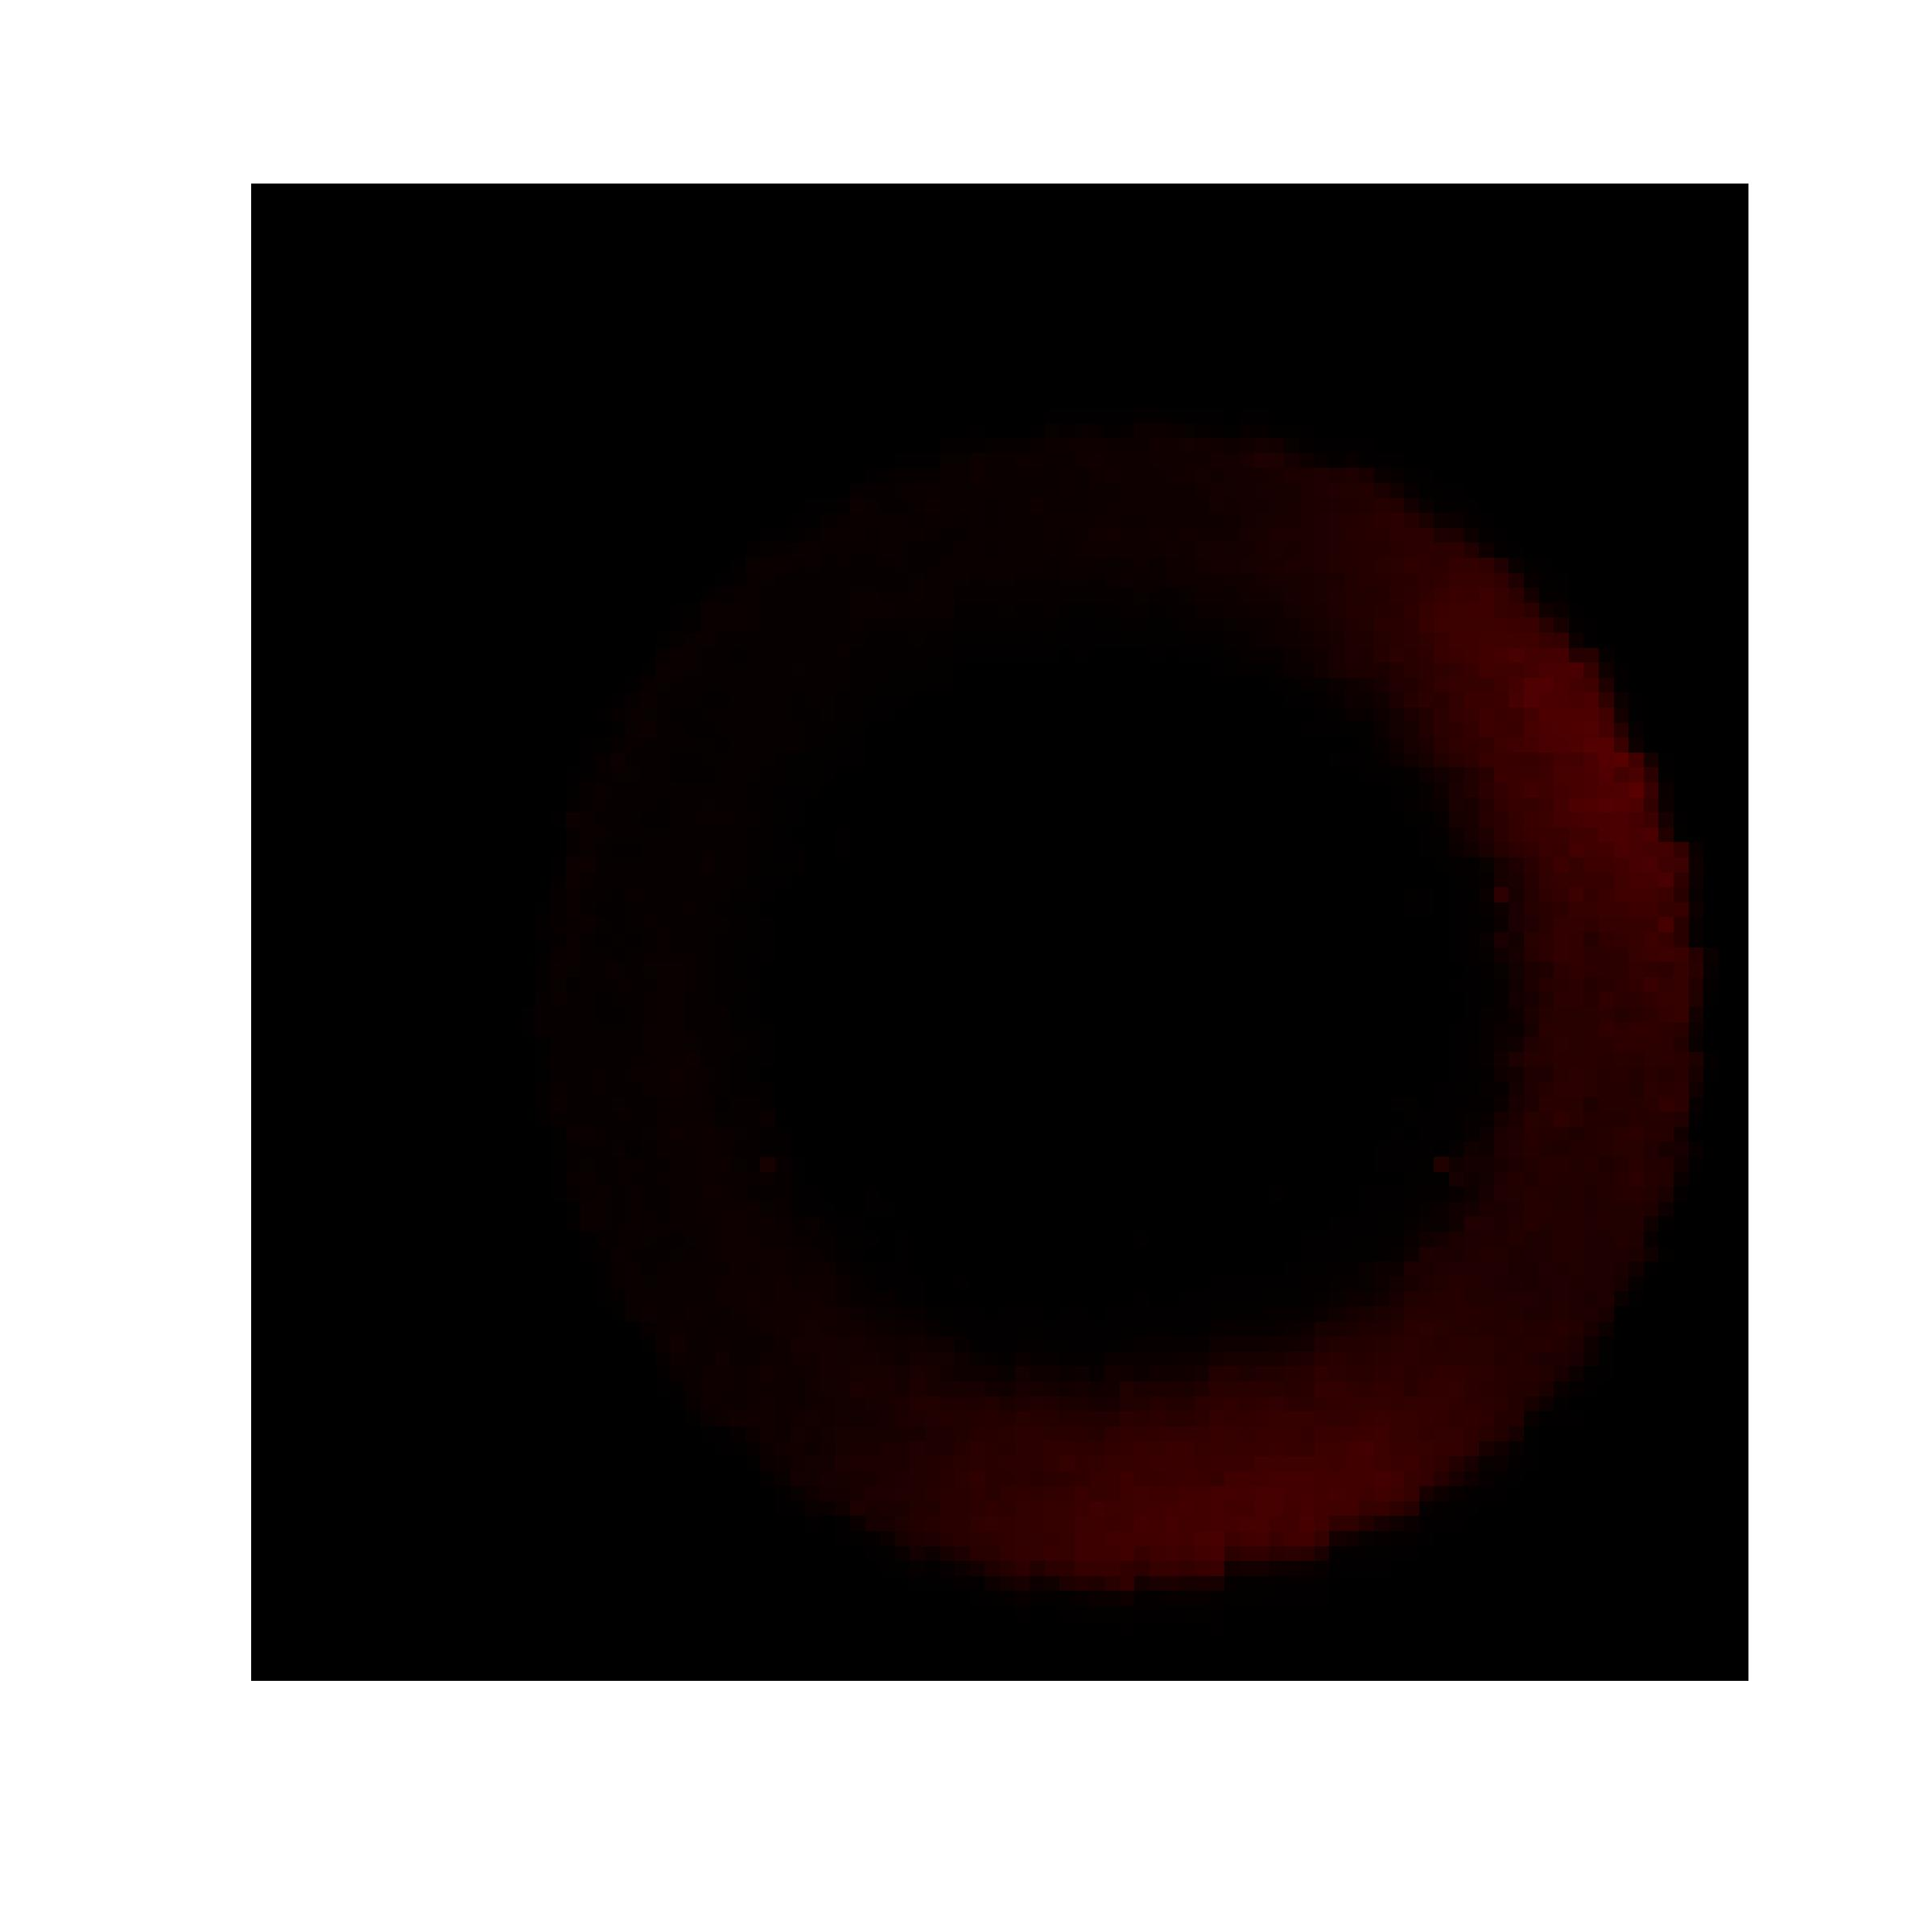
\includegraphics[width=0.15\textwidth]{dpERK_vdm_3}
    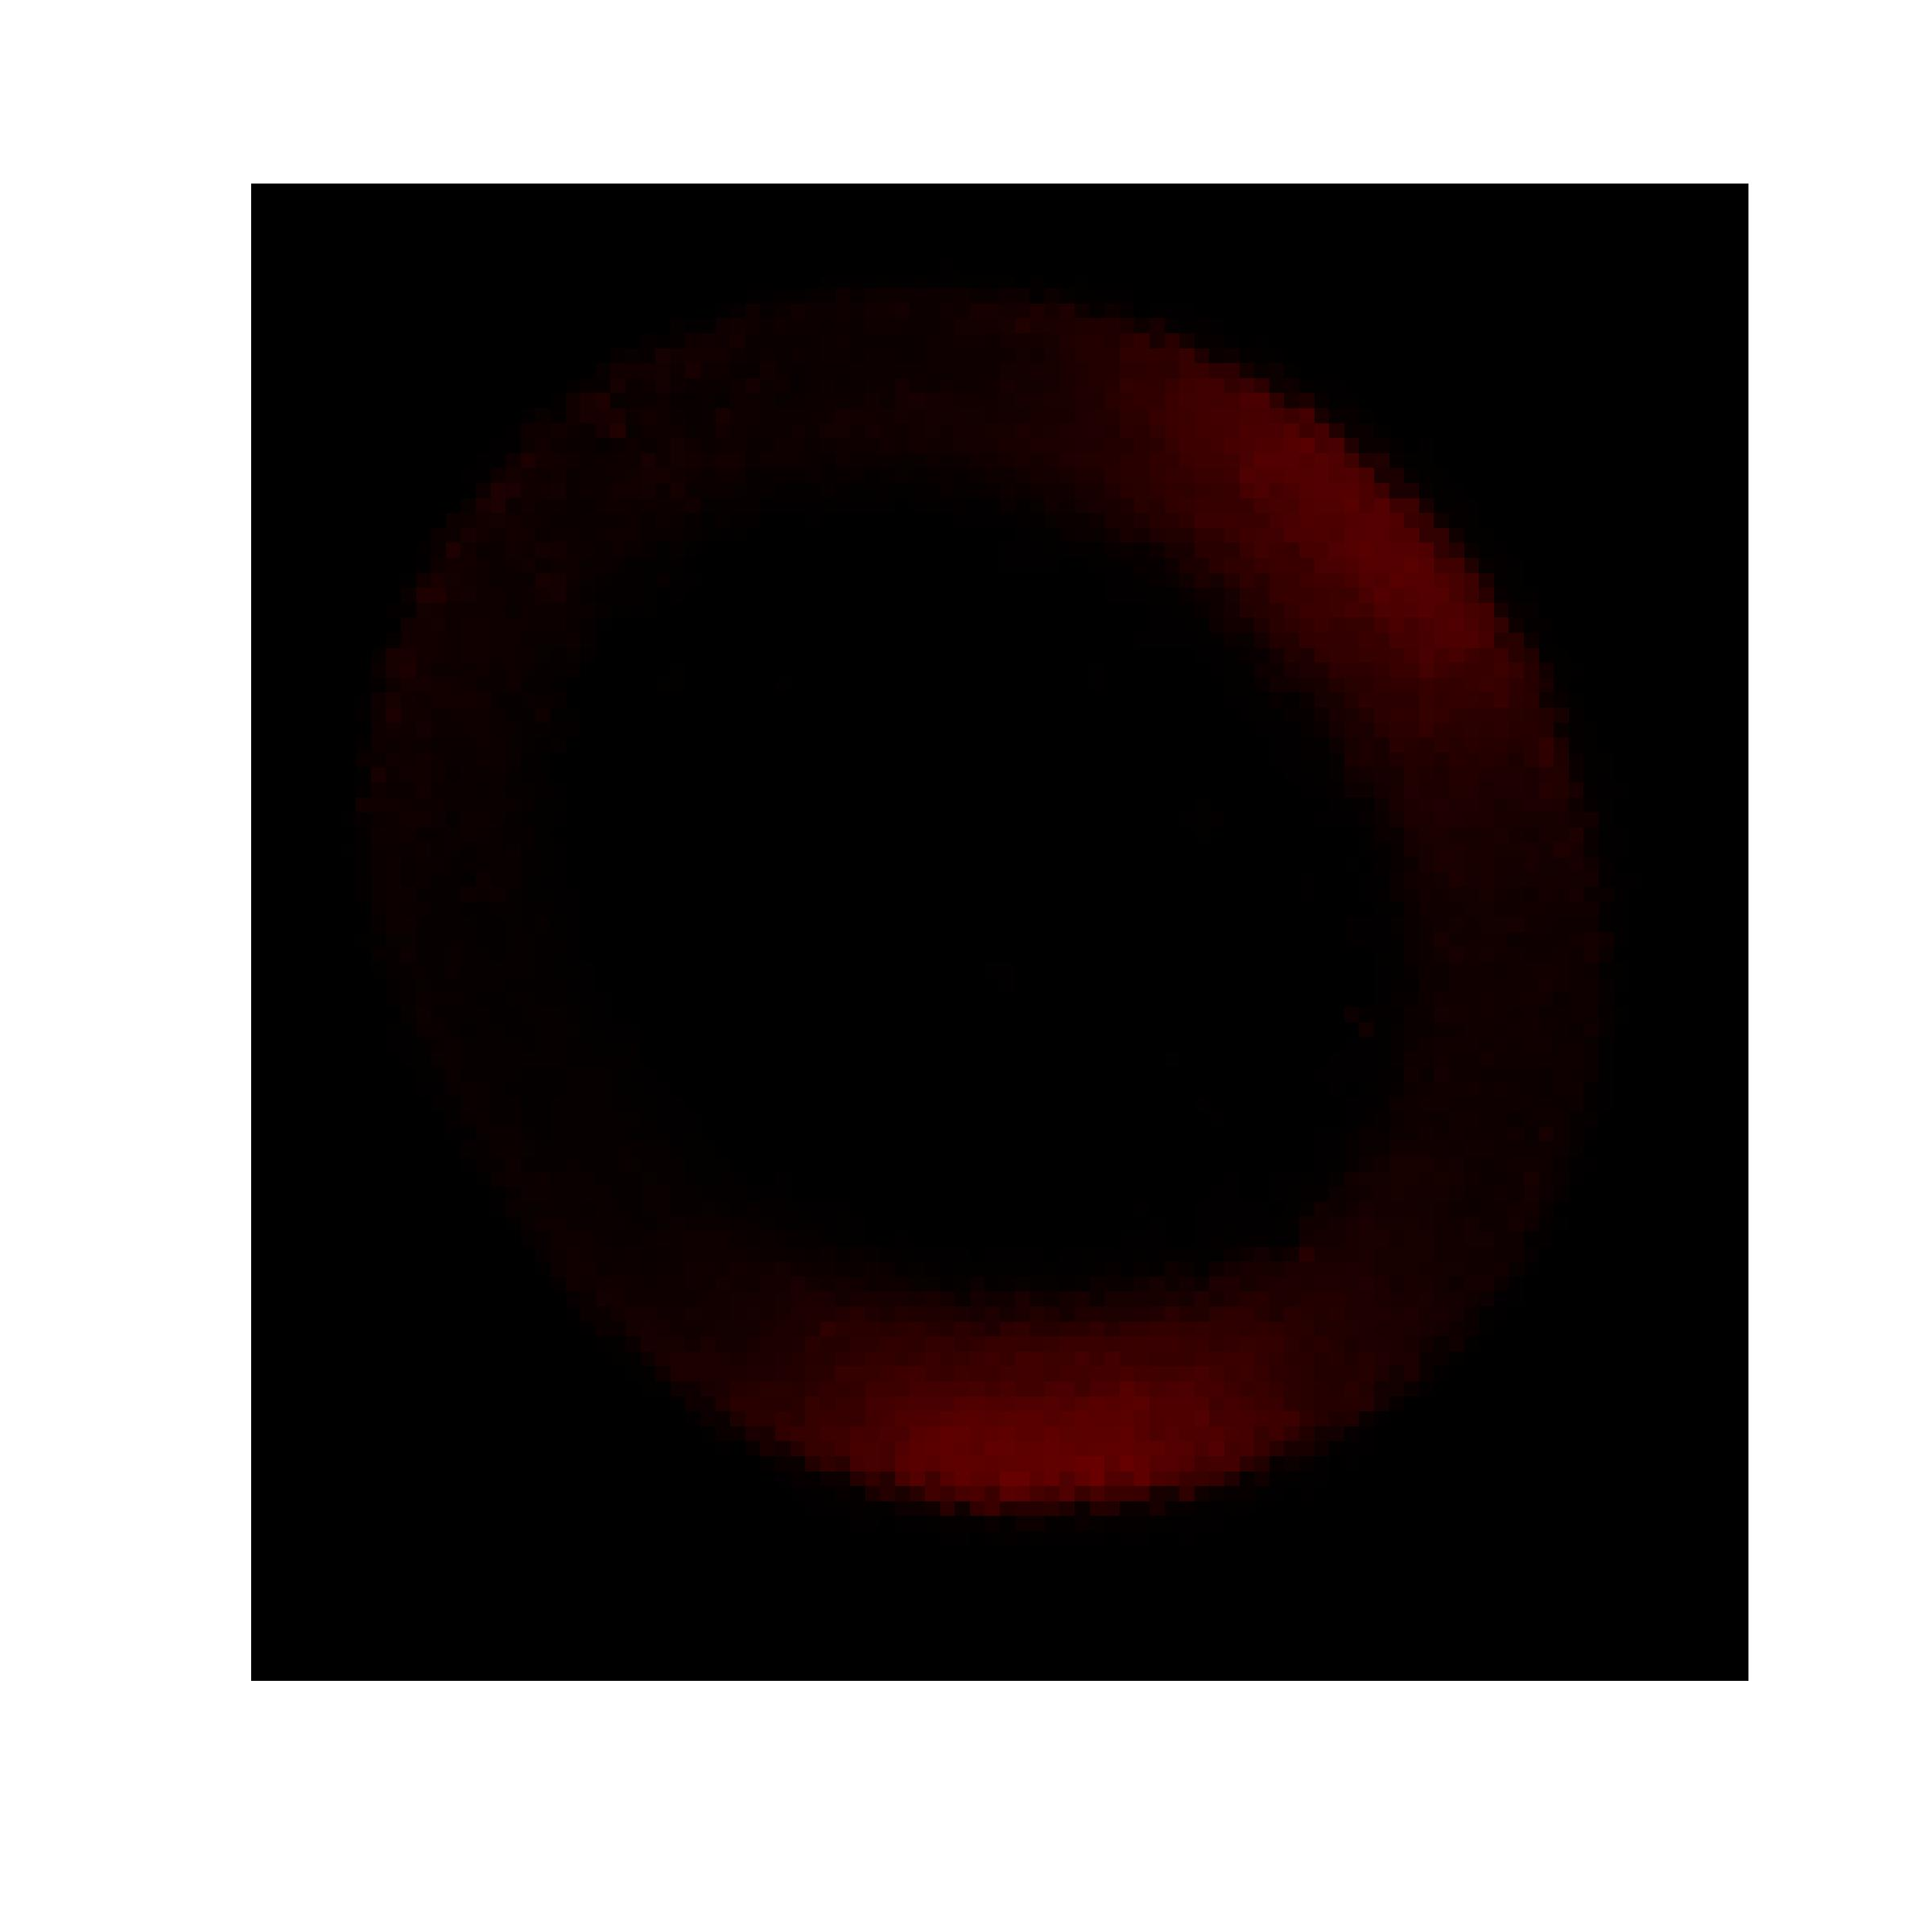
\includegraphics[width=0.15\textwidth]{dpERK_vdm_4}
    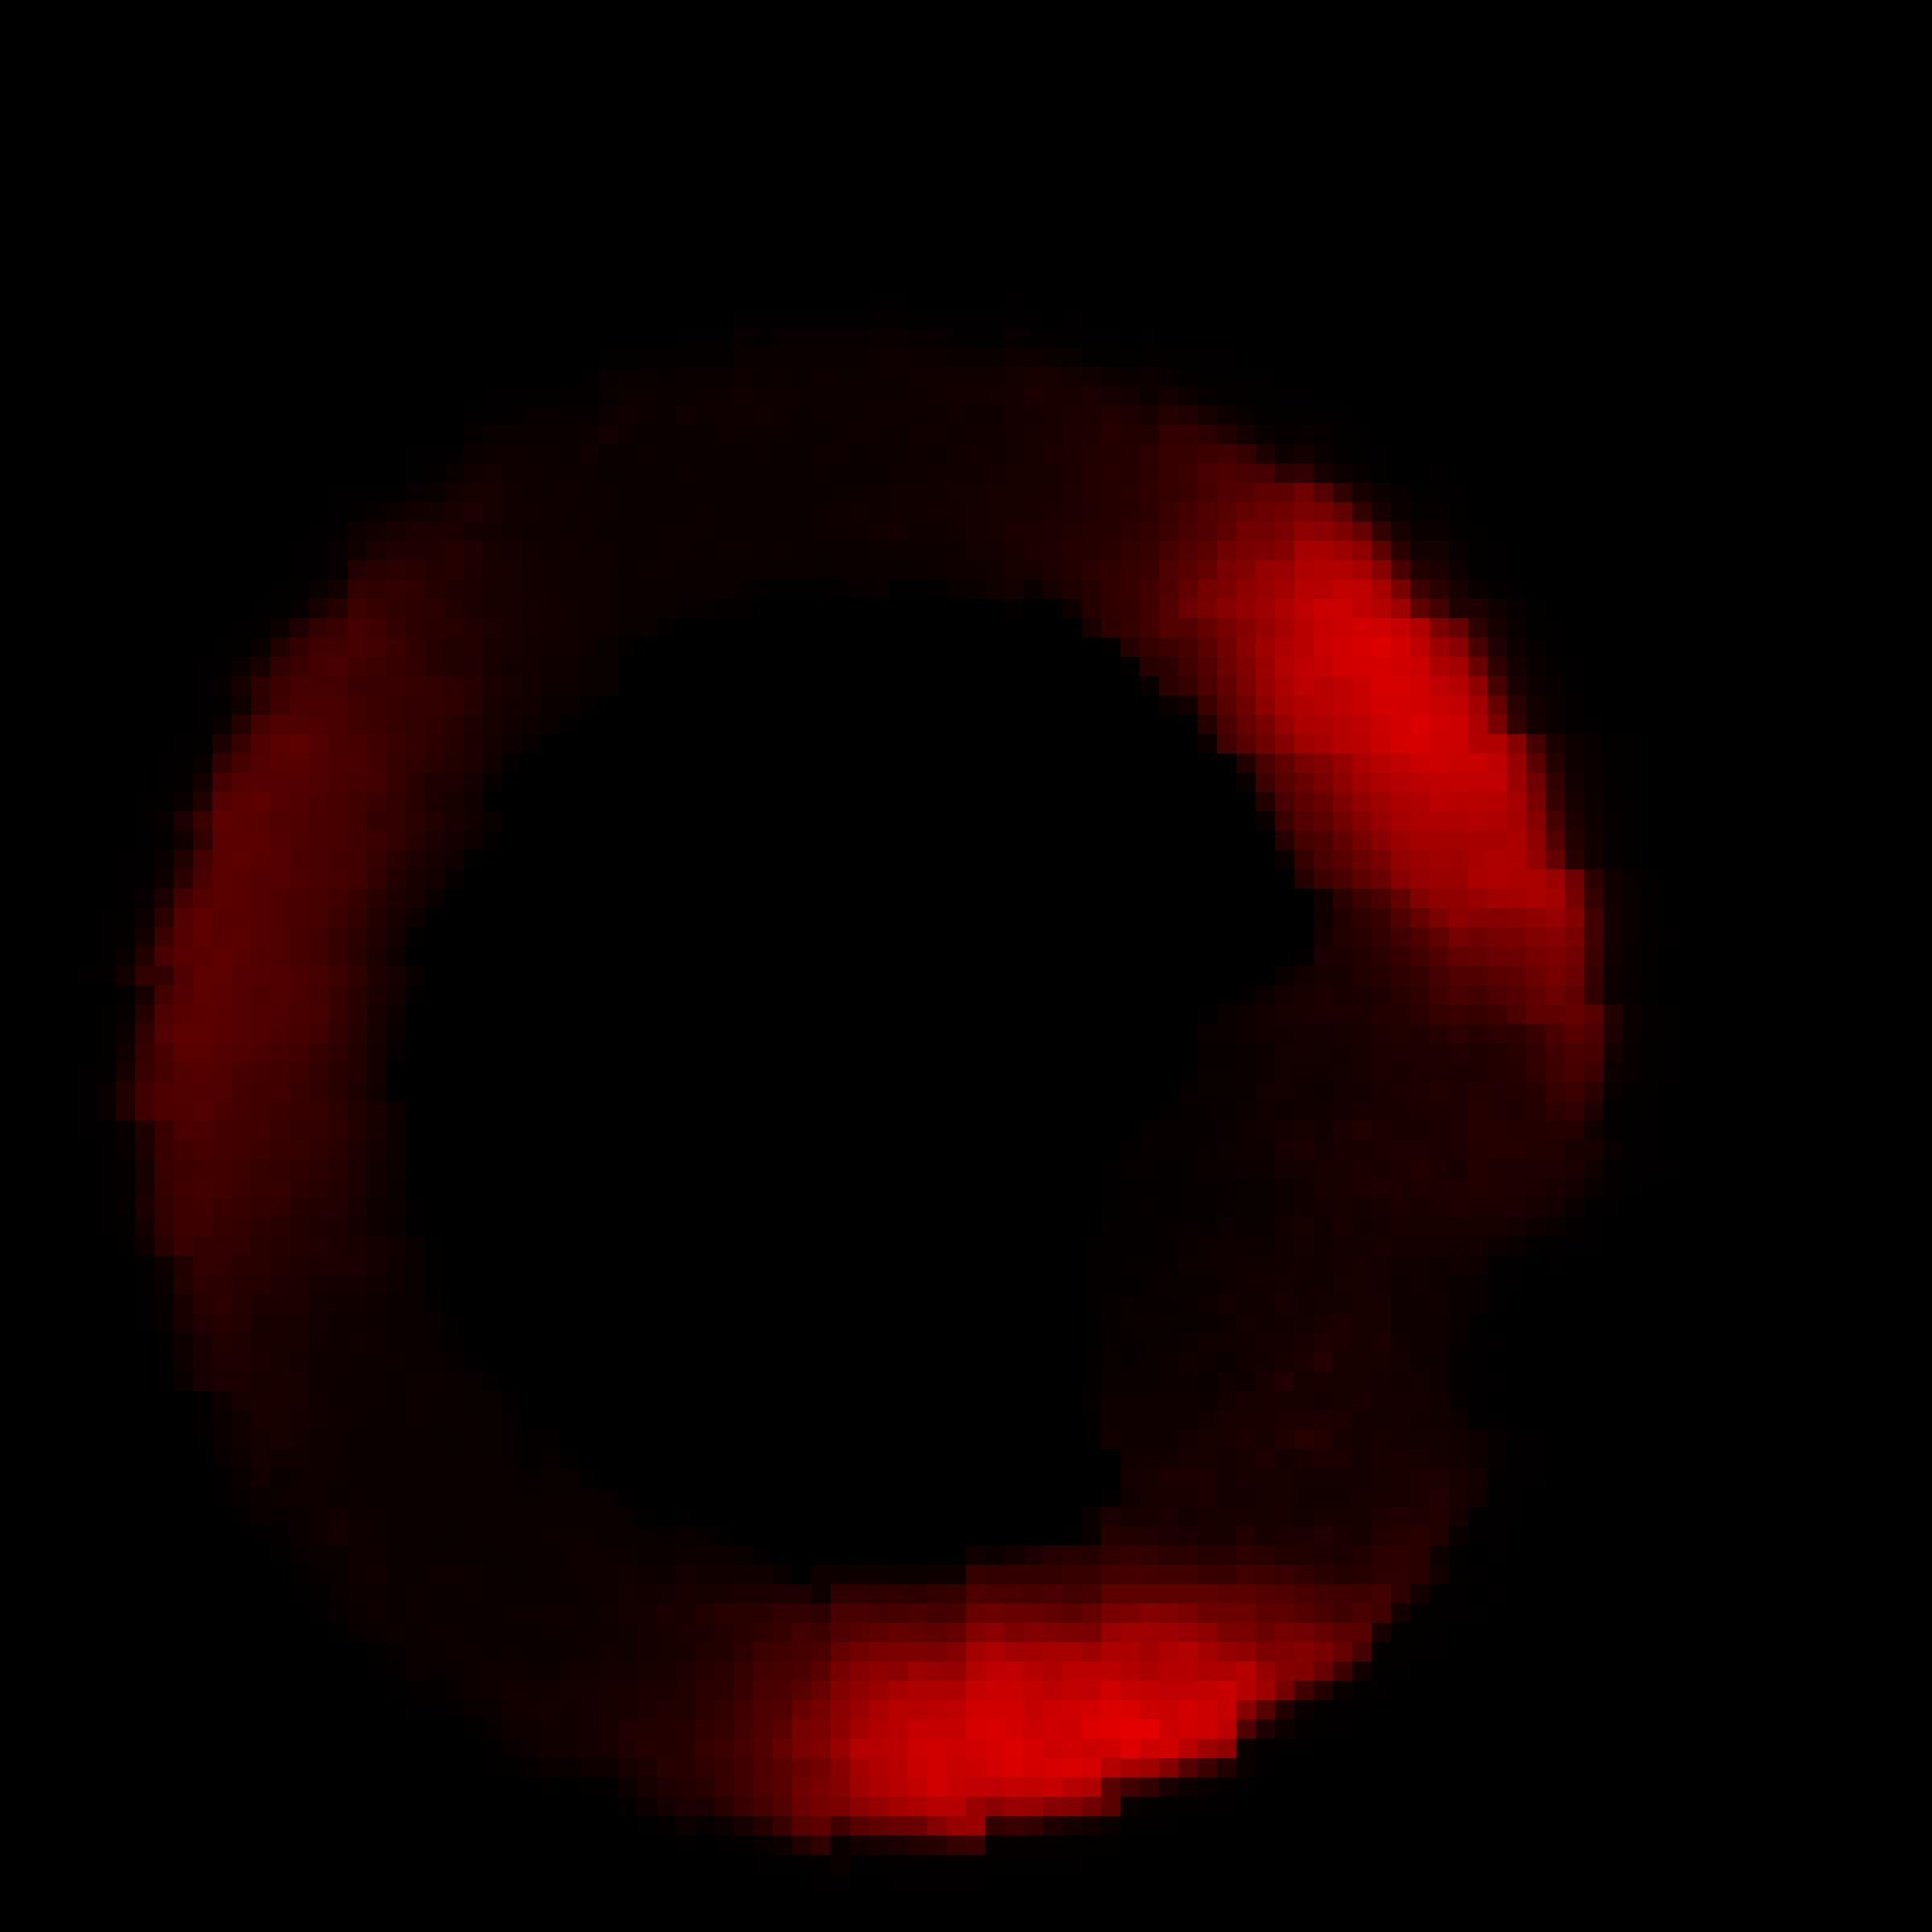
\includegraphics[width=0.15\textwidth]{dpERK_vdm_5}
    
\end{frame}

\begin{frame}{Alignment of Two-Dimensional Images}
    We first align and order the images using the scattering transform\\
    
    \centering
    
\includegraphics[width=0.5\textwidth]{DMAPS_scat_time_corr}\\
    
\includegraphics[width=0.15\textwidth]{dpERK_scat_1}
    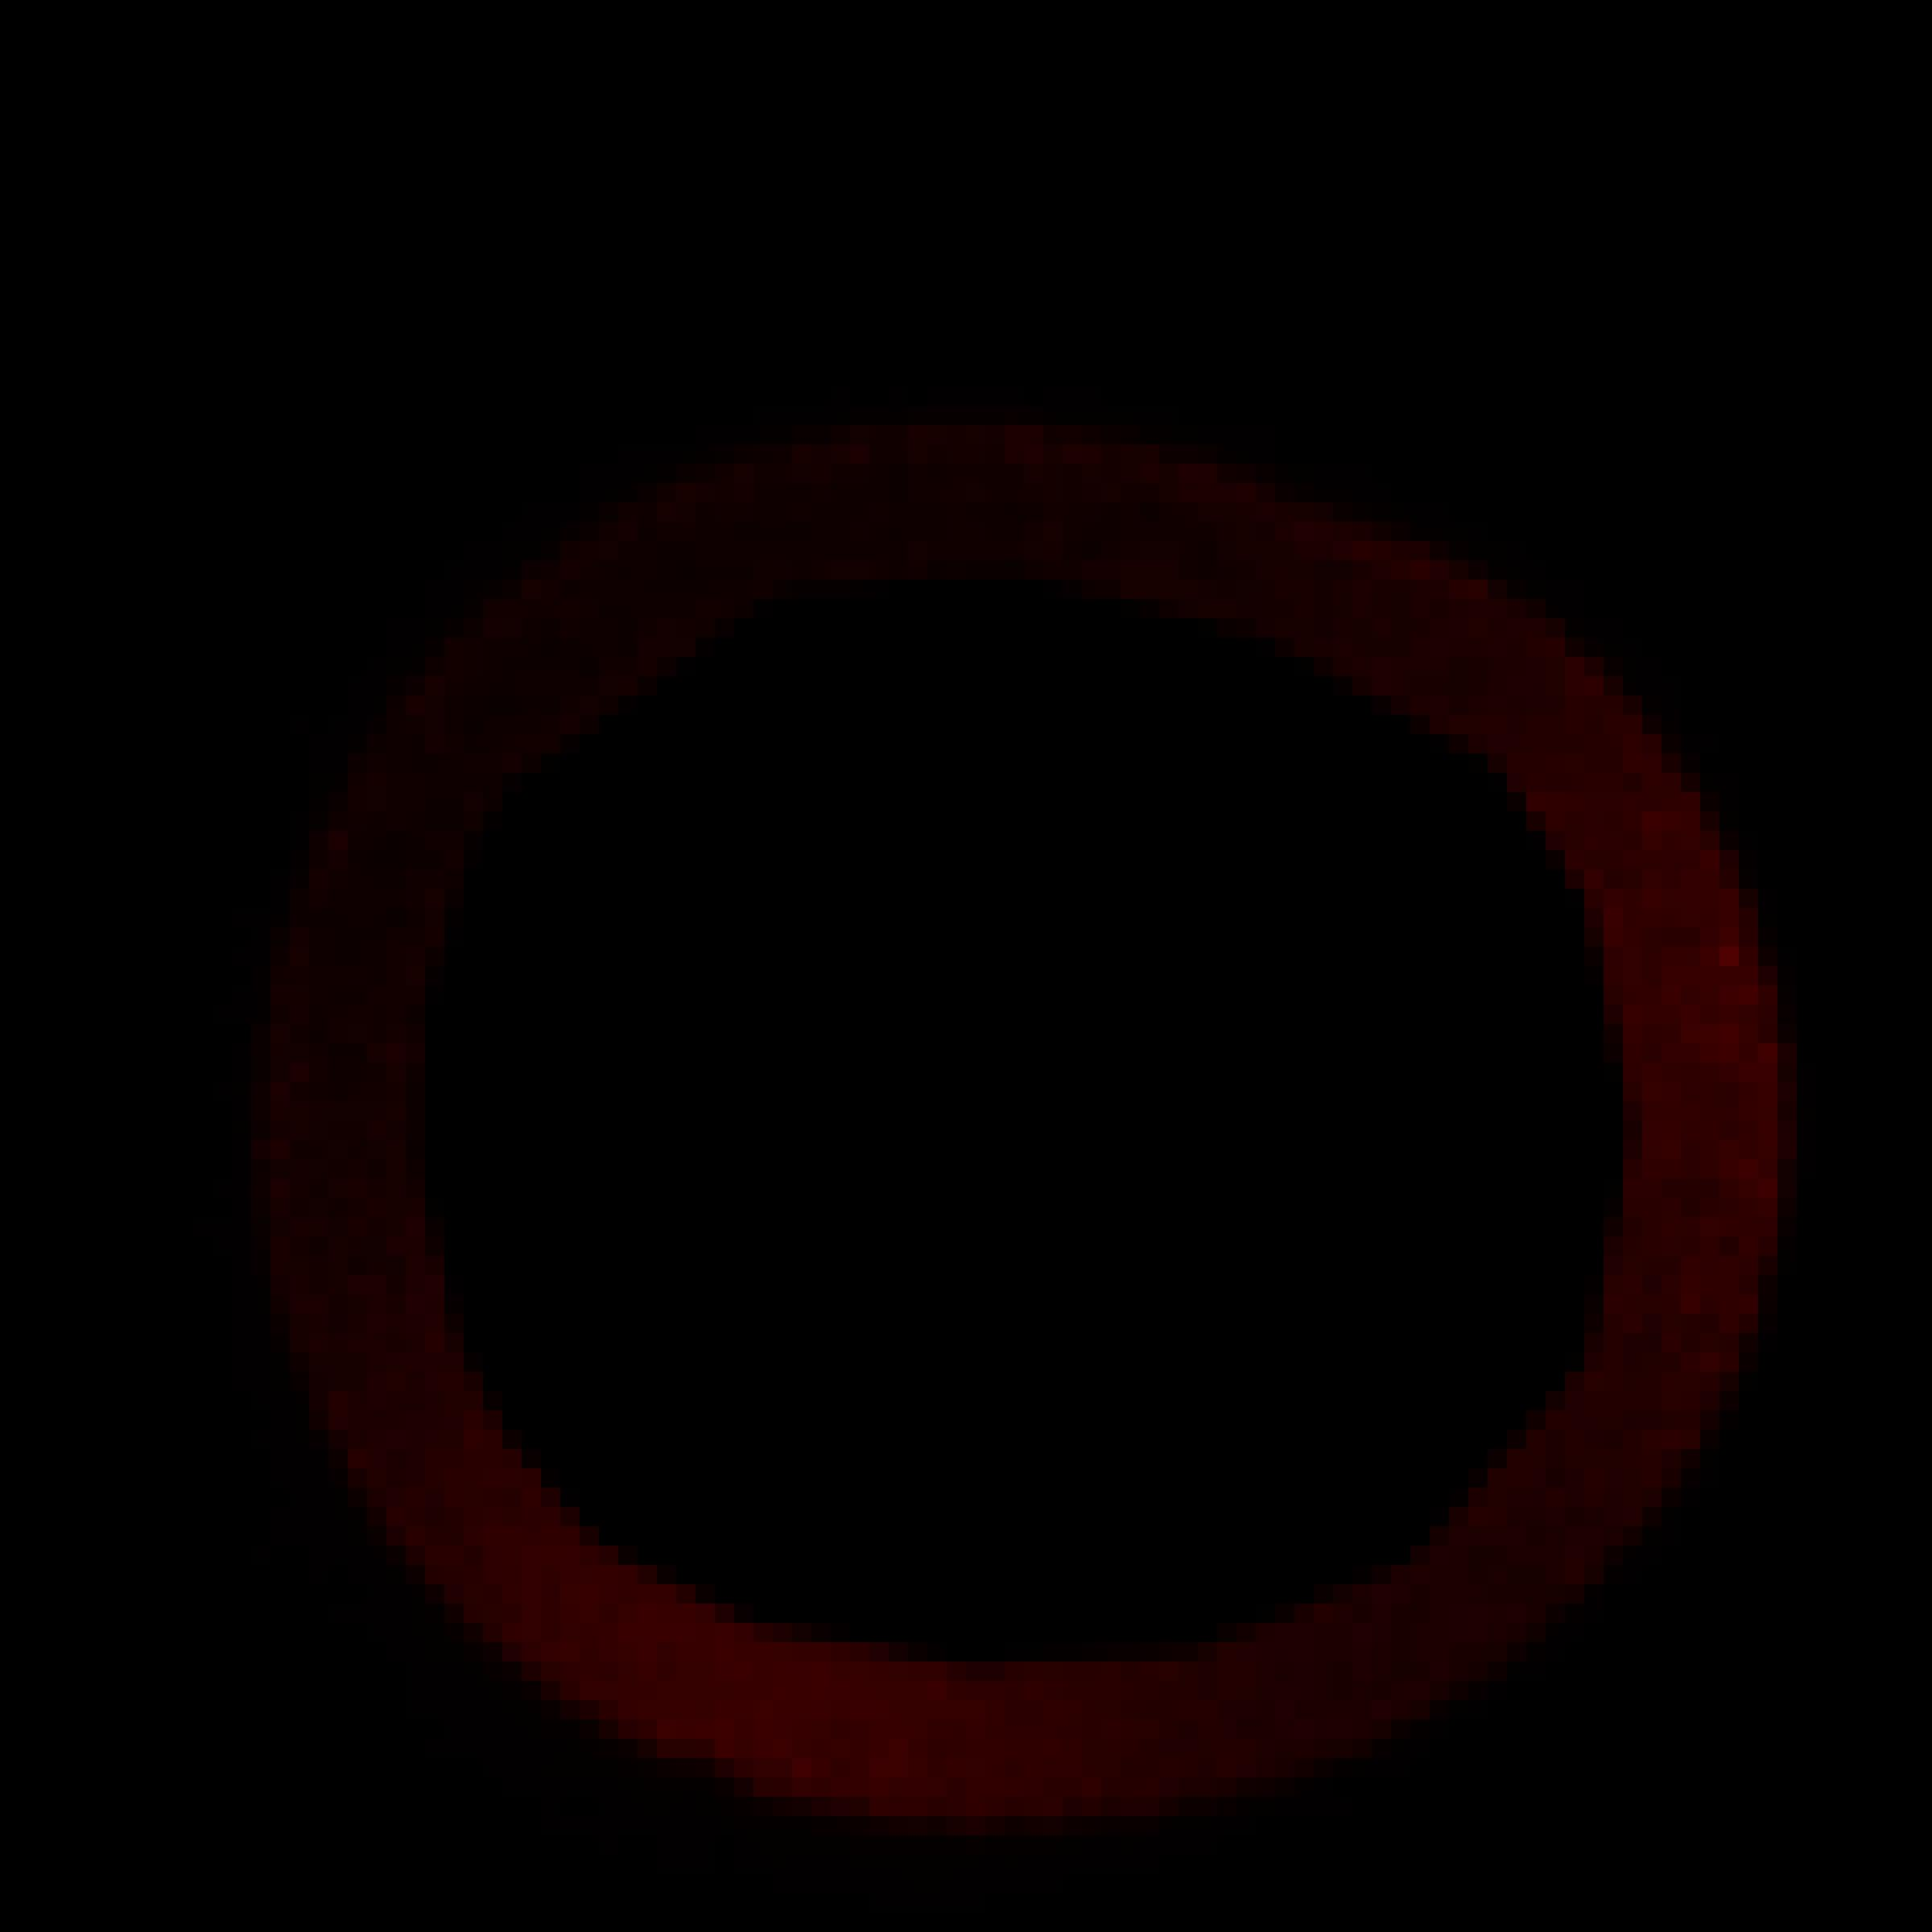
\includegraphics[width=0.15\textwidth]{dpERK_scat_2}
    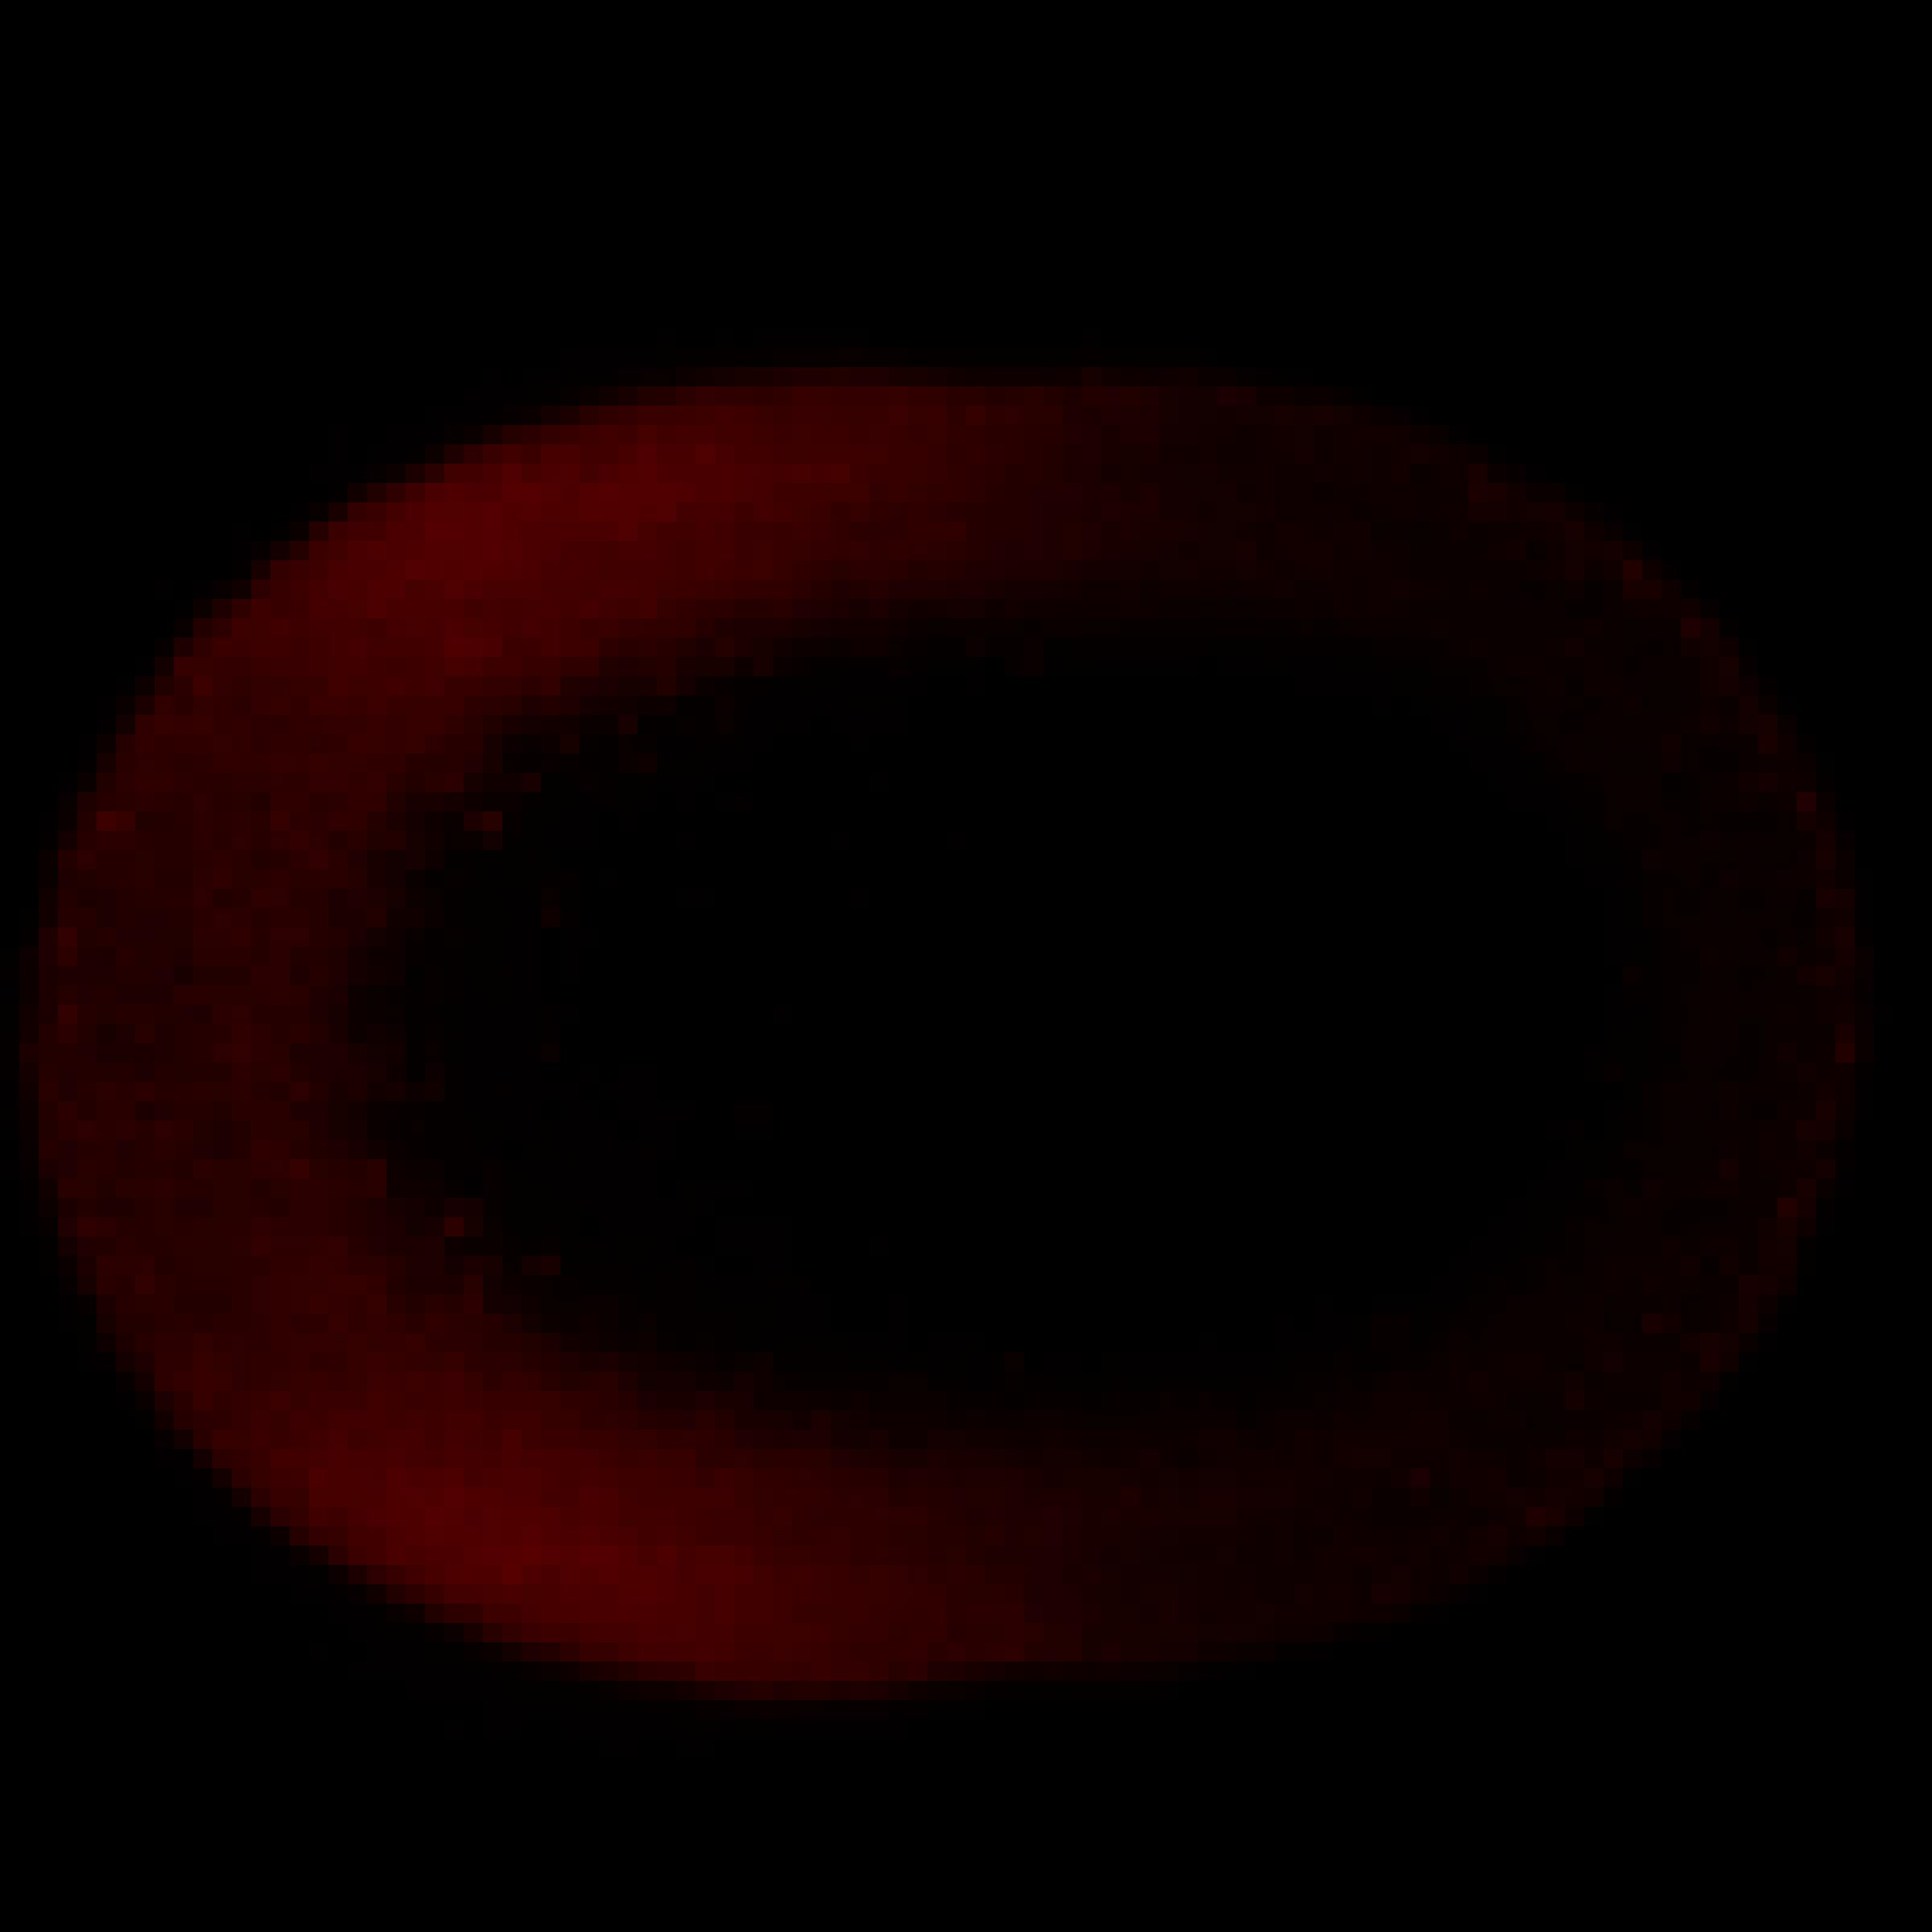
\includegraphics[width=0.15\textwidth]{dpERK_scat_3}
    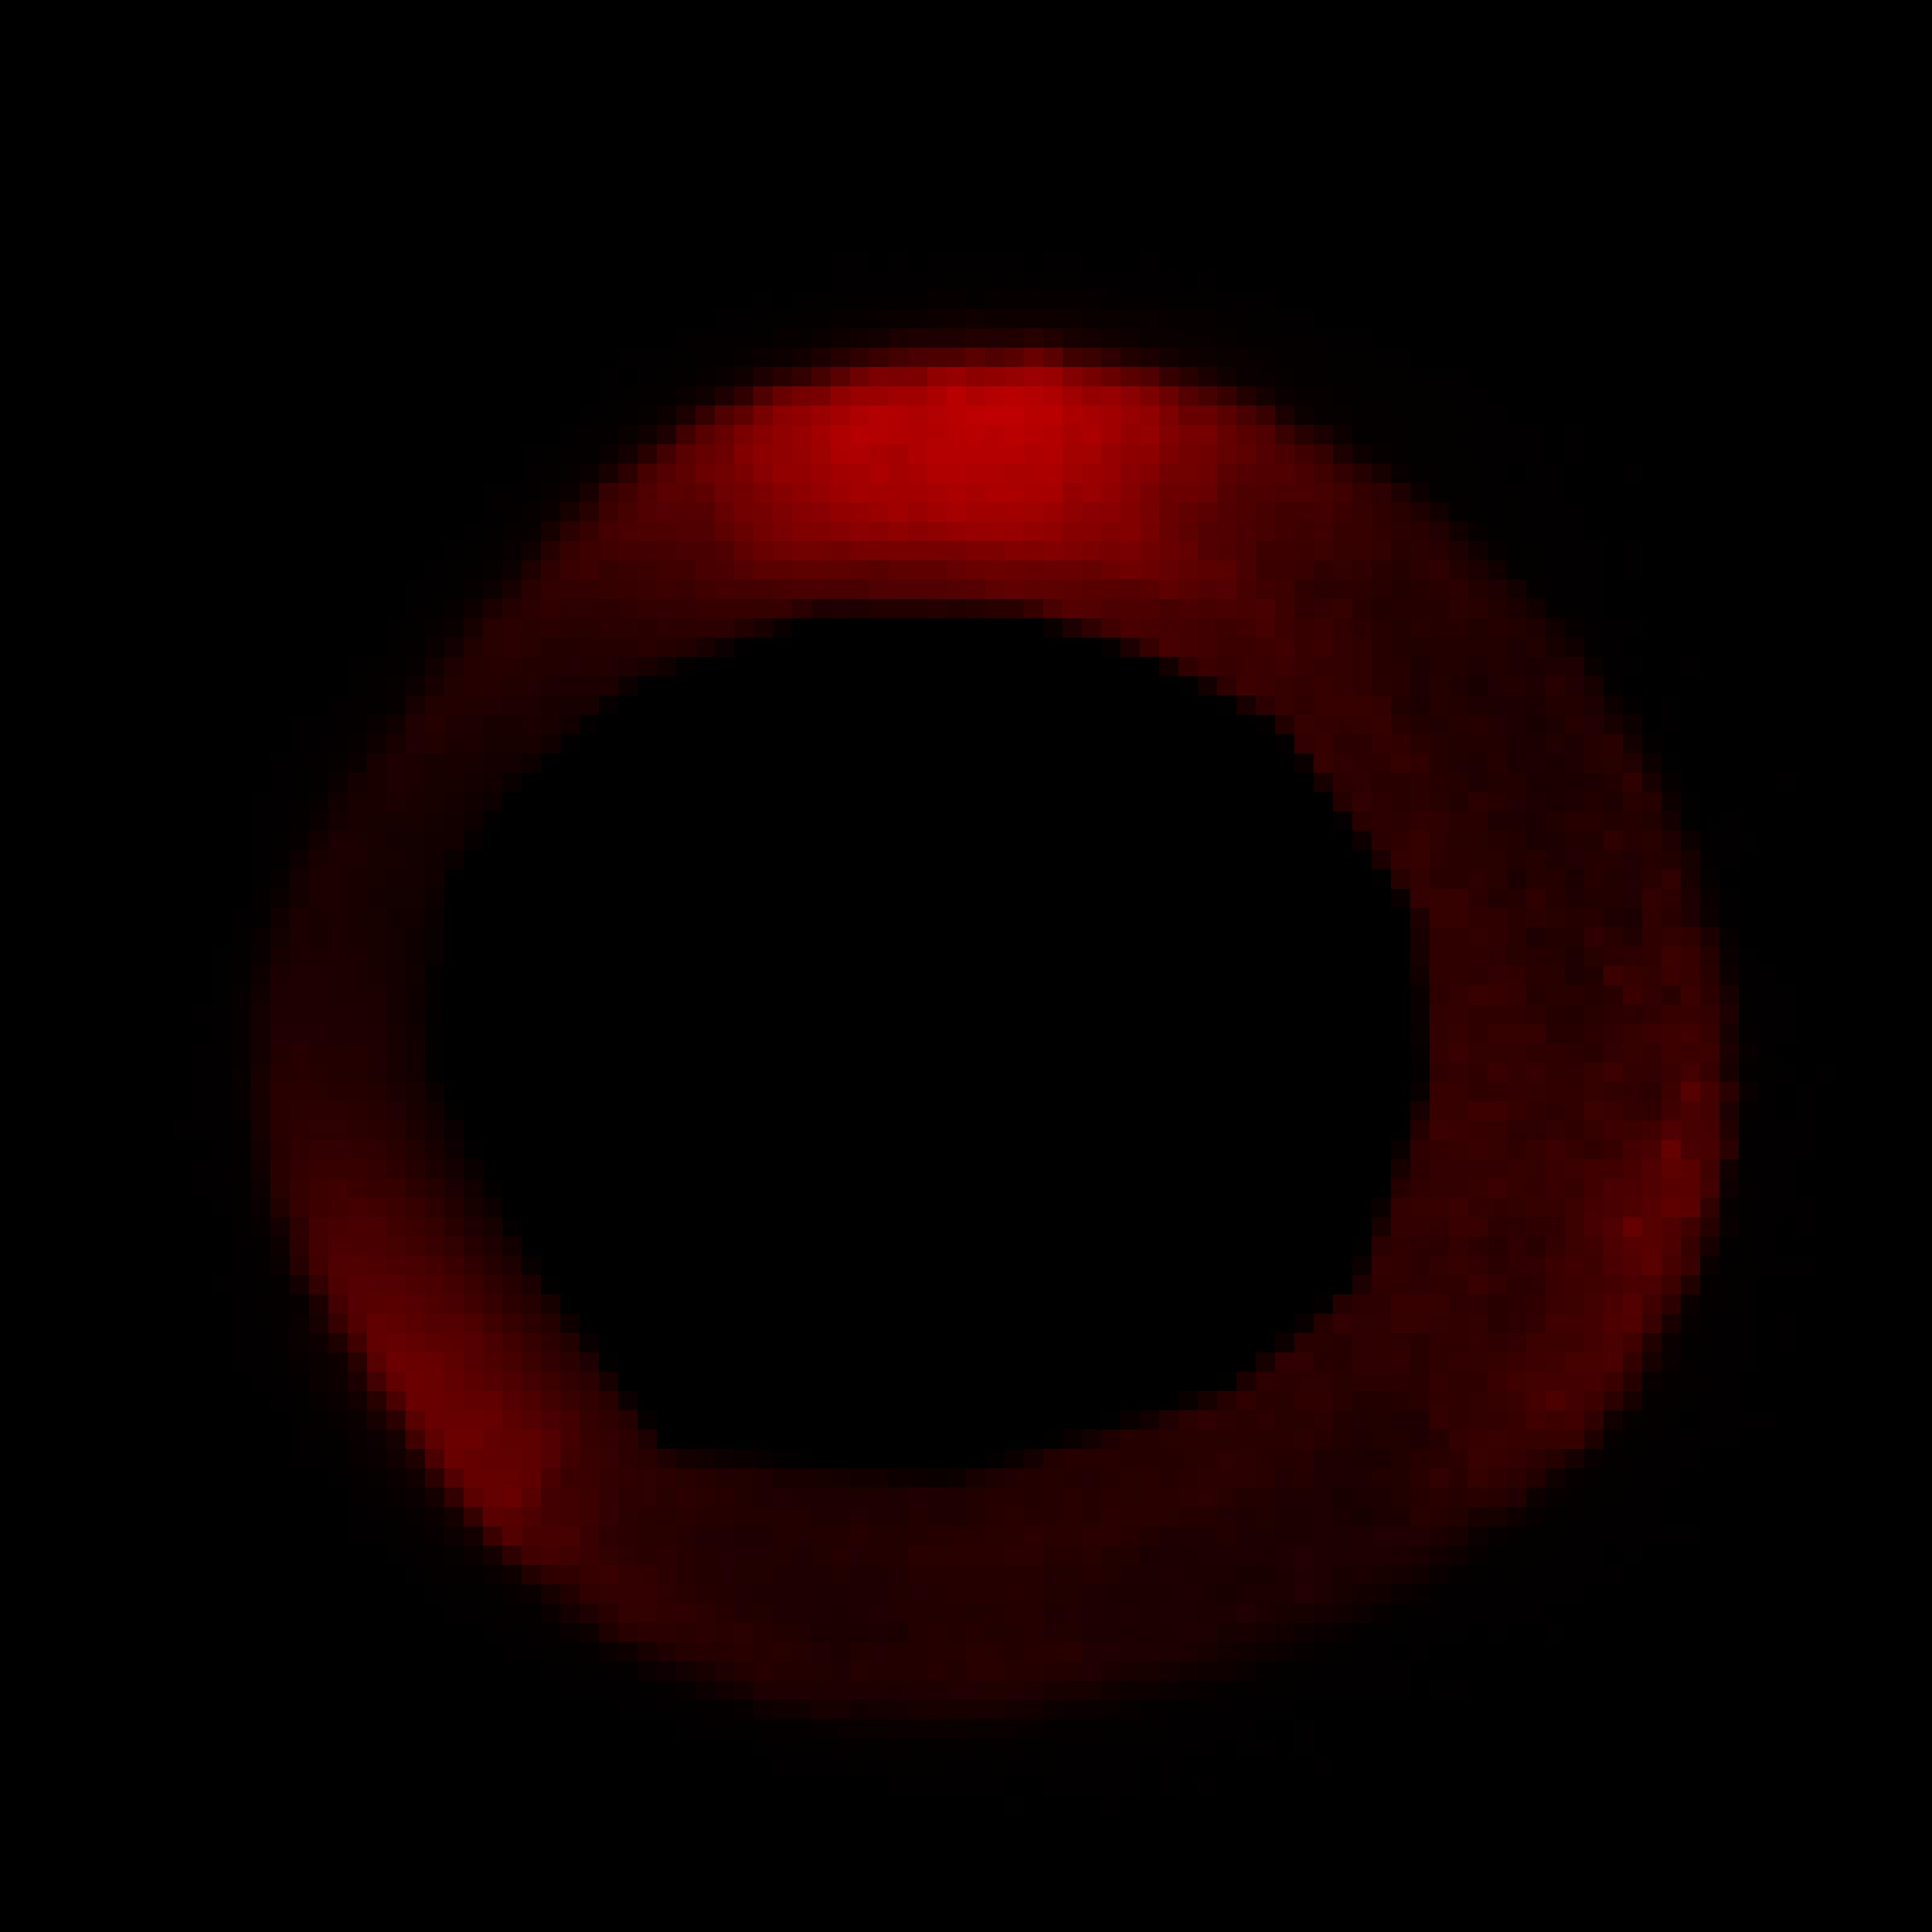
\includegraphics[width=0.15\textwidth]{dpERK_scat_4}
    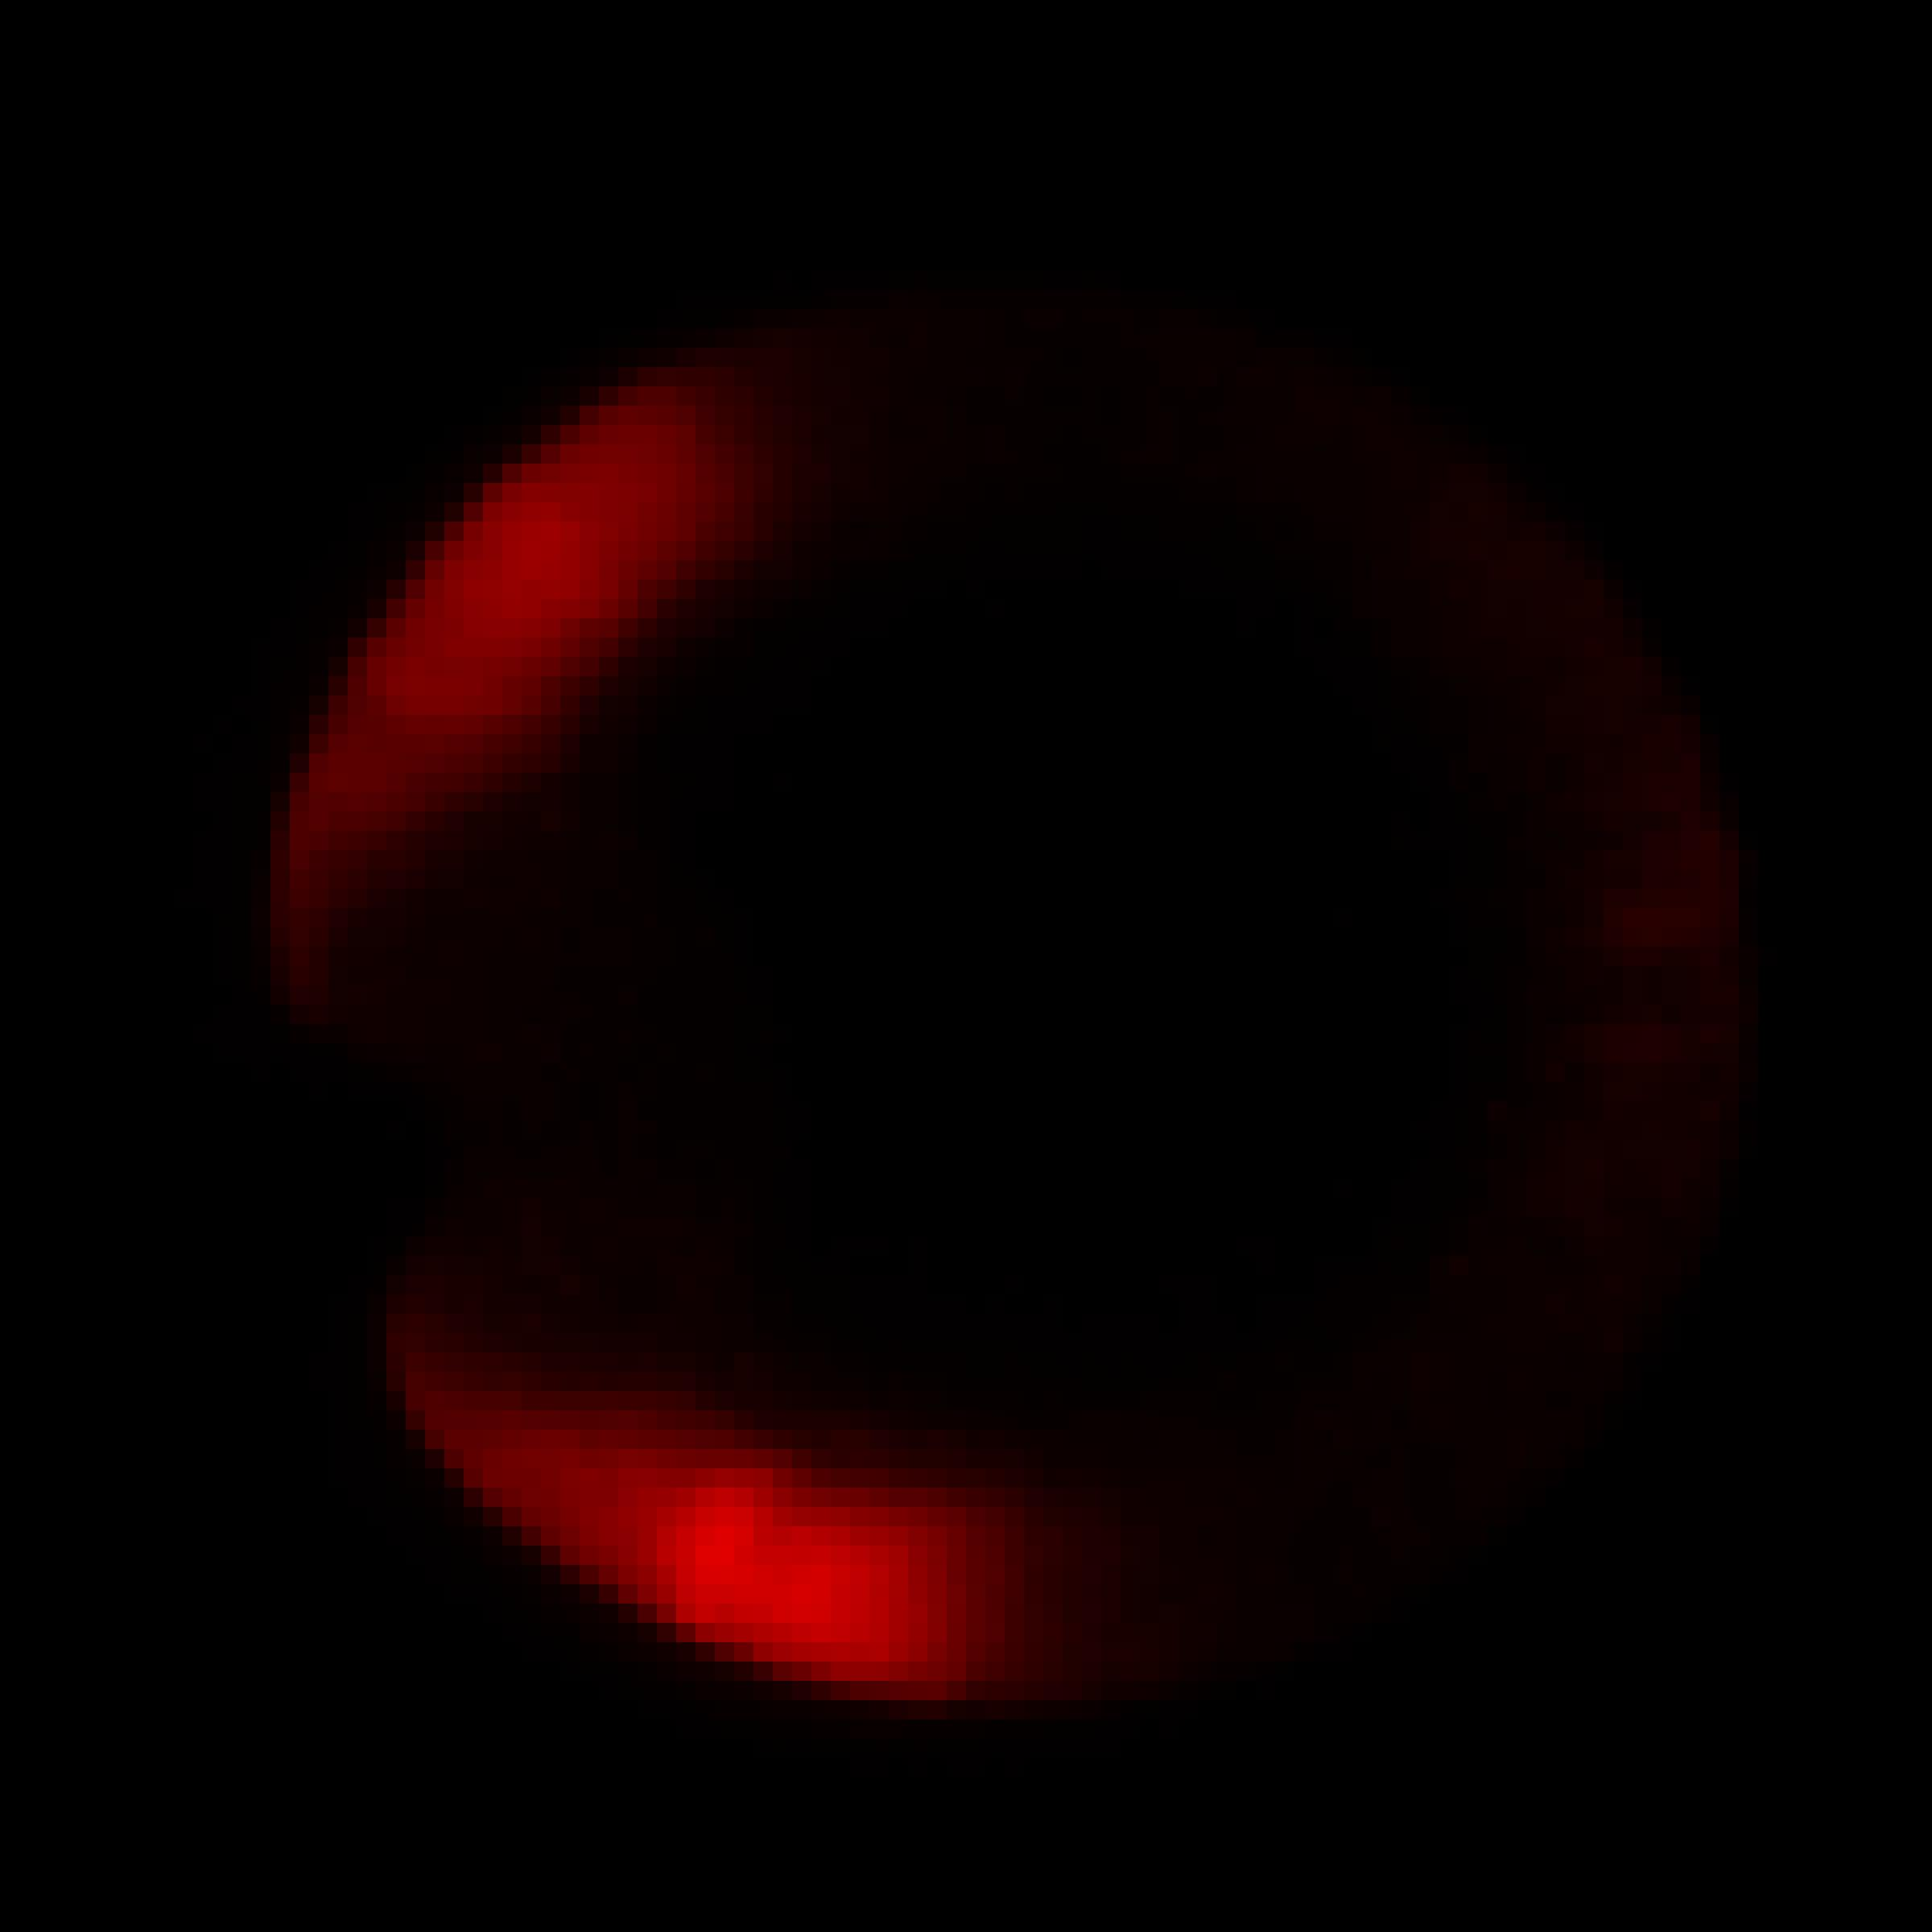
\includegraphics[width=0.15\textwidth]{dpERK_scat_5}
    
\end{frame}

    
    

    